\documentclass[12pt]{article}

% --- 1. CONFIGURACIÓN BASE Y TIPOGRAFÍA ---
\usepackage[utf8]{inputenc}
\usepackage[spanish]{babel}
\usepackage{helvet}
\renewcommand{\familydefault}{\sfdefault}
\usepackage[left=2.5cm,right=2.5cm,top=3cm,bottom=3cm]{geometry}
\usepackage{parskip}
\usepackage{titlesec}
\usepackage{blindtext}

% --- 2. GESTIÓN DE COLORES ---
\usepackage{xcolor}
\definecolor{pastelblue}{RGB}{31, 110, 165}
\newcommand{\correccion}[1]{\textcolor{pastelblue}{#1}}
% Comando personalizado para comentarios
\newcommand{\VPcomment}[1]{\textcolor{purple}{\textbf{[VP:} #1\textbf{]}}}

% --- 3. GESTIÓN DE IMÁGENES Y FIGURAS ---
\usepackage{graphicx}
\usepackage{float}
% Rutas donde LaTeX buscará las imágenes
\graphicspath{{figures/}{img/tensiones/}{img/cargabilidad/}{img/general/}{img/}}

% --- 4. GESTIÓN DE TABLAS Y PAISAJE ---
\usepackage{array}
\usepackage{multirow}
\usepackage{longtable}
\usepackage{booktabs}
\usepackage{makecell}
\usepackage{threeparttable}
\usepackage{pdflscape}

% --- 5. ENCABEZADOS Y PIES DE PÁGINA ---
\usepackage{fancyhdr}
\setlength{\headheight}{2cm}
\renewcommand{\headrulewidth}{0pt}
\renewcommand{\footrulewidth}{0pt}
\pagestyle{fancy}

% Configuración del encabezado Izquierdo
\lhead{%
    \fbox{%
        \begin{minipage}[t][2.2cm][c]{.23\linewidth}%
            \begin{center}
                
\includegraphics[width=1.6cm]{LogoVDD.png}\\
                CONTRATO No:
            \end{center}
        \end{minipage}%
    }% end \fbox
}% end \lhead

% Configuración del encabezado Central
\chead{%
    \fbox{%
        \begin{minipage}[t][2.2cm][c]{.5\linewidth}%
            \begin{center}
                \textbf{Informe}\\
                \textbf{Escuela de Ingeniería Eléctrica, Electrónica y Telecomunicaciones – UIS}\\
                \textbf{CONSTRUCCIÓN DEL SEGMENTO DE POTENCIA DEL ÁREA SANTANDER}\\
            \end{center}
        \end{minipage}%
    }% end \fbox
}% end \chead

% Configuración del encabezado Derecho
\rhead{%
    \fbox{%
        \begin{minipage}[t][2.2cm][c]{.23\linewidth}%
            \begin{center}
                \textbf{Revisión: 1}\\
                \vspace{5mm}
                \textbf{Página \thepage{} de \pageref*{LastPage}}
            \end{center}
        \end{minipage}%
    }% end \fbox
}% end \rhead

% --- 6. HIPERVÍNCULOS Y METADATOS PDF (Debe ir casi siempre al final) ---
\usepackage{hyperref}
\hypersetup{
    colorlinks,
    citecolor=black,
    filecolor=black,
    linkcolor=black,
    urlcolor=black
}
\pdfgentounicode=1
\usepackage{lastpage}

% ==========================================
% COMIENZA EL DOCUMENTO
% ==========================================
\begin{document}

\begin{center}
\phantom{This text will be invisible} \\
\vspace{1.5cm}
Informe N°1\\
Escuela de Ingeniería Eléctrica, Electrónica y Telecomunicaciones – UIS.\\
\vspace{4cm}
CONSTRUCCIÓN DEL SEGMENTO DE POTENCIA DEL ÁREA SANTANDER.\\
\vspace{4cm}
Elaborado por:\\
Dairo Alexander Lobo Moreno\\
Daniel Fernando Aranda Contreras\\
Yulieth Valentina Portilla Jaimes\\

\vspace{4cm}
Dependencia que desarrolla el informe\\
PROELCO\\
Bucaramanga, 14 de septiembre de 2023.\\
\vspace{2cm}
\end{center}
\newpage
\phantom{This text will be invisible} \\

\begin{table}[h]
\centering
\begin{tabular}{|ccc|}
\hline
\multicolumn{3}{|c|}{ÍNDICE DE REVISIONES}                                                                \\ \hline
\multicolumn{1}{|c|}{Índice revisión} & \multicolumn{1}{c|}{Fecha modificación} & Modificaciones \\ \hline
\multicolumn{1}{|c|}{0}               & \multicolumn{1}{c|}{}                   &                \\ \hline
\multicolumn{1}{|c|}{1}               & \multicolumn{1}{c|}{}                   &                \\ \hline
\end{tabular}
\end{table}

\begin{table}[h]
\centering
\begin{tabular}{|cc|c|c|}
\hline
\multicolumn{2}{|c|}{Versión}                            & 0 & 1 \\ \hline
\multicolumn{1}{|c|}{\multirow{2}{*}{Ejecuta}}  & Nombre &   &   \\ \cline{2-4}
\multicolumn{1}{|c|}{}                          & Fecha  &   &   \\ \hline
\multicolumn{1}{|c|}{\multirow{2}{*}{Revisa}}   & Nombre &   &   \\ \cline{2-4}
\multicolumn{1}{|c|}{}                          & Fecha  &   &   \\ \hline
\multicolumn{1}{|c|}{\multirow{2}{*}{Verifica}} & Nombre &   &   \\ \cline{2-4}
\multicolumn{1}{|c|}{}                          & Fecha  &   &   \\ \hline
\multicolumn{1}{|c|}{\multirow{2}{*}{Aprueba}}  & Nombre &   &   \\ \cline{2-4}
\multicolumn{1}{|c|}{}                          & Fecha  &   &   \\ \hline
\end{tabular}
\end{table}

\newpage
\vspace*{0.1cm}
\renewcommand\contentsname{Tabla de contenido}
\tableofcontents
\newpage
\vspace*{0.1cm}
\renewcommand{\listfigurename}{Lista de figuras}
\listoffigures
\newpage
\vspace*{0.1cm}
\renewcommand{\listtablename}{Lista de tablas}
\listoftables
\newpage
\vspace*{0.1cm}

\section{Resumen ejecutivo}
El presente Estudio de Ajuste y Coordinación de Protecciones (EACP) tiene como propósito evaluar la viabilidad técnica y el comportamiento eléctrico asociado a la integración progresiva de las Etapas N.° 1 y N.° 2 del proyecto \textit{Construcción del Segmento de Potencia del Área Santander} al Sistema Interconectado Nacional (SIN). Para ello, se realizaron simulaciones de flujo de carga y cortocircuito en el software DIgSILENT PowerFactory, considerando escenarios de demanda mínima y máxima. El análisis comprendió las subestaciones de Piedecuesta, Mesa del Sol, San Gil, Cabrera, Oiba, Suaita, Barbosa y Guatiguará, con el fin de evaluar los perfiles de tensión, la cargabilidad de los elementos y los niveles de corriente de cortocircuito antes y después de la incorporación del proyecto. Los resultados del flujo de carga permitieron identificar que, durante la Etapa N.° 1, se presentaban condiciones de baja tensión en las subestaciones de Barbosa, Suaita, Oiba, Cabrera y San Gil, siendo la condición más crítica la registrada en la barra de Barbosa 115 kV, con un valor de 0.849 p.u. Como medida correctiva, se determinó la necesidad de incorporar un banco de capacitores de 22.5 MVAr a 115 kV en la subestación Barbosa. Con la implementación de esta compensación y la posterior incorporación de la Etapa N.° 2, los niveles de tensión del sistema se mantuvieron dentro de los límites operativos establecidos, entre 0.95 p.u. y 1.05 p.u., sin presentarse elementos con cargabilidades superiores al 100\% de su capacidad nominal. Por otra parte, el análisis de cortocircuito mostró que las fallas trifásicas (3F) producen las mayores magnitudes de corriente simétrica inicial ($I_k''$). La mayor corriente de falla del modelo se presentó en los bornes de la Central Sogamoso a 16.5 kV, con valores superiores a 240 kA. En el nivel de 220 kV, la mayor corriente se registró en la subestación Guatiguará, alcanzando 58.6 kA, mientras que para el nivel de 115 kV los valores más elevados se presentaron en las subestaciones Bucaramanga y Piedecuesta. Al comparar los niveles de cortocircuito entre las diferentes etapas del proyecto, se observó que la mayor variación se concentra en Piedecuesta, con incrementos entre 10.1\% y 12.2\%, debido a su ubicación como punto de acople de la nueva red. En las demás subestaciones, especialmente aquellas más alejadas del proyecto, las variaciones fueron reducidas, llegando a ser inferiores al 0.03\%. A partir de los resultados obtenidos, se establece que la incorporación de las Etapas N.° 1 y N.° 2 del proyecto es técnicamente viable bajo las condiciones analizadas, considerando la implementación de la compensación reactiva de 22.5 MVAr en la subestación Barbosa 115 kV. Esta medida permite mejorar las condiciones de tensión del área y, junto con los resultados de flujo de carga y cortocircuito, proporciona los elementos técnicos necesarios para la posterior revisión y ajuste de los esquemas de protección asociados al área de estudio.

\section{Objetivo}
Evaluar el comportamiento eléctrico y la viabilidad técnica de la integración de las Etapas N$^\circ$ 1 y N$^\circ$ 2 del proyecto ``Construcción del Segmento de Potencia del Área Santander'' al Sistema Interconectado Nacional (SIN), mediante la simulación de flujos de potencia y el análisis de corrientes de falla bajo escenarios de demanda mínima y máxima, con el fin de diagnosticar la regulación de tensión, cuantificar los niveles de cortocircuito en las nuevas subestaciones (Piedecuesta 115 kV, Mesa del Sol 115 kV, San Gil 115 kV, Cabrera 115 kV, Oiba 115 kV, Suaita 115 kV, Barbosa 115 kV y Cabrera 220 kV) y determinar el impacto operativo y los aportes de falla sobre los nodos existentes y subestaciones adyacentes del área de influencia.

\section{Alcance}
El presente estudio técnico, correspondiente a la fase de análisis eléctricos de soporte para el Estudio de Ajuste y Coordinación de Protecciones (EACP), comprende la modelación y evaluación de las condiciones operativas para la integración progresiva de las Etapas N.° 1 y N.° 2 del proyecto de expansión del Área Santander al Sistema Interconectado Nacional (SIN). Empleando un modelo de red ajustado a las condiciones de operación del SIN, la delimitación del área de influencia parte de las barras adyacentes a los puntos de conexión del proyecto, extendiéndose o contrayéndose de acuerdo con los criterios de influencia eléctrica definidos por el Consejo Nacional de Operación (CNO). En esta fase se ejecutarán los estudios de flujo de carga y cortocircuito para las configuraciones de red de cada etapa. El análisis de flujo de carga permitirá evaluar los perfiles de tensión y la cargabilidad de los elementos para identificar restricciones operativas y, ante desviaciones de la regulación de tensión, establecer la necesidad y las características de la compensación reactiva requerida. Por su parte, el estudio de cortocircuito comprende el cálculo de corrientes de falla para cortocircuitos francos (\(0\,\Omega\)) de tipo monofásico, bifásico a tierra, bifásico y trifásico, bajo los escenarios de demanda máxima y mínima definidos para el estudio. Los resultados obtenidos constituirán los insumos técnicos para la posterior revisión, ajuste y coordinación de los sistemas de protección asociados a los elementos nuevos, reconfigurados o impactados por el proyecto, incluyendo las líneas de transmisión a 115 kV y 220 kV, el transformador Cabrera 220/115 kV y las instalaciones asociadas a las subestaciones de frontera Piedecuesta, Barbosa y Guatiguará. En consecuencia, esta fase se limita a los estudios de soporte de flujo de carga y cortocircuito, por lo que no comprende la parametrización final de relés ni las verificaciones detalladas de selectividad, las cuales serán desarrolladas en las etapas posteriores del EACP.

\section{Documentos consultados}
Para establecer los criterios de evaluación empleados en el análisis, se consultó el Concepto CREG 246 de 2024, del cual se adoptó como referencia que las tensiones en las barras de 110 kV, 115 kV, 220 kV y 230 kV deben mantenerse entre el 90 \% y el 110 \% de la tensión nominal. Se consultó la información comercial de EPRECSA para identificar las alternativas disponibles de bancos de capacitores y seleccionar el equipo comercial utilizado como referencia para la compensación reactiva del proyecto. Se utilizaron los datos disponibles en XM – Sinergox para determinar las condiciones de demanda mínima, media y máxima empleadas en las simulaciones del sistema.

\section{Descripción del proyecto}

\subsection{Etapas del proyecto}
El proyecto de expansión de la red de transmisión del Área Santander se desarrolla en \textbf{dos etapas de puesta en servicio}, mediante la incorporación progresiva de nueva infraestructura al sistema de potencia. Para cada etapa se describe la infraestructura prevista y se presenta su respectiva configuración topológica.

\textbf{Etapa N.° 1.} La Etapa N.° 1 comprende la incorporación de la infraestructura de transmisión a 115 kV conformada por los enlaces Piedecuesta 115 kV--Mesa del Sol 115 kV, Mesa del Sol 115 kV--San Gil 115 kV, San Gil 115 kV--Cabrera 115 kV, Cabrera 115 kV--Oiba 115 kV, Oiba 115 kV--Suaita 115 kV y Suaita 115 kV--Barbosa 115 kV. Adicionalmente, contempla la conexión entre Cabrera 115 kV y Cabrera 220 kV mediante el transformador de potencia correspondiente. \textbf{Fecha esperada de entrada en operación:} 22 de abril de 2027. La configuración topológica correspondiente a esta etapa se presenta en la Figura~\ref{fig:etapa1}.

\begin{figure}[H]
    \centering
    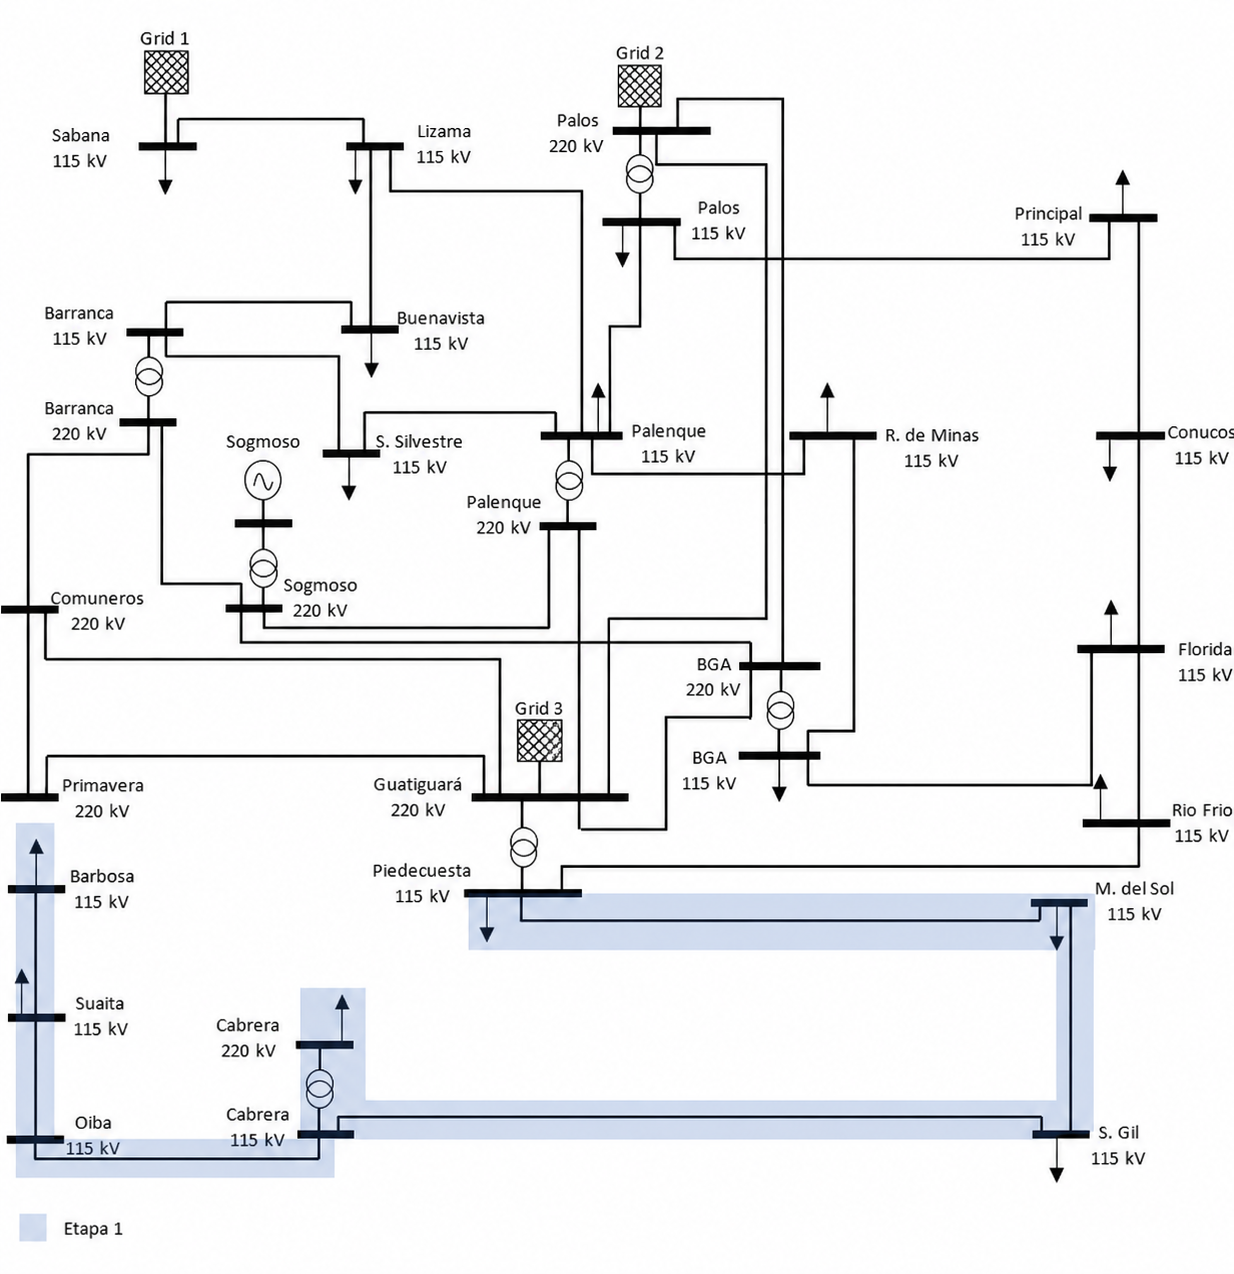
\includegraphics[width=0.65\linewidth]{etapa1.png}
    \caption{Sistema de potencia en estudio: Etapa N.° 1.}
    \label{fig:etapa1}
\end{figure}

\textbf{Etapa N.° 2.} La Etapa N.° 2 comprende la infraestructura incorporada durante la Etapa N.° 1 y adiciona el enlace de transmisión Cabrera 220 kV--Guatiguará 220 kV. Esta conexión constituye la infraestructura adicional prevista para la segunda etapa del proyecto. \textbf{Fecha esperada de entrada en operación:} 22 de abril de 2027. La configuración topológica correspondiente a esta etapa se presenta en la Figura~\ref{fig:etapa2}.

\begin{figure}[H]
    \centering
    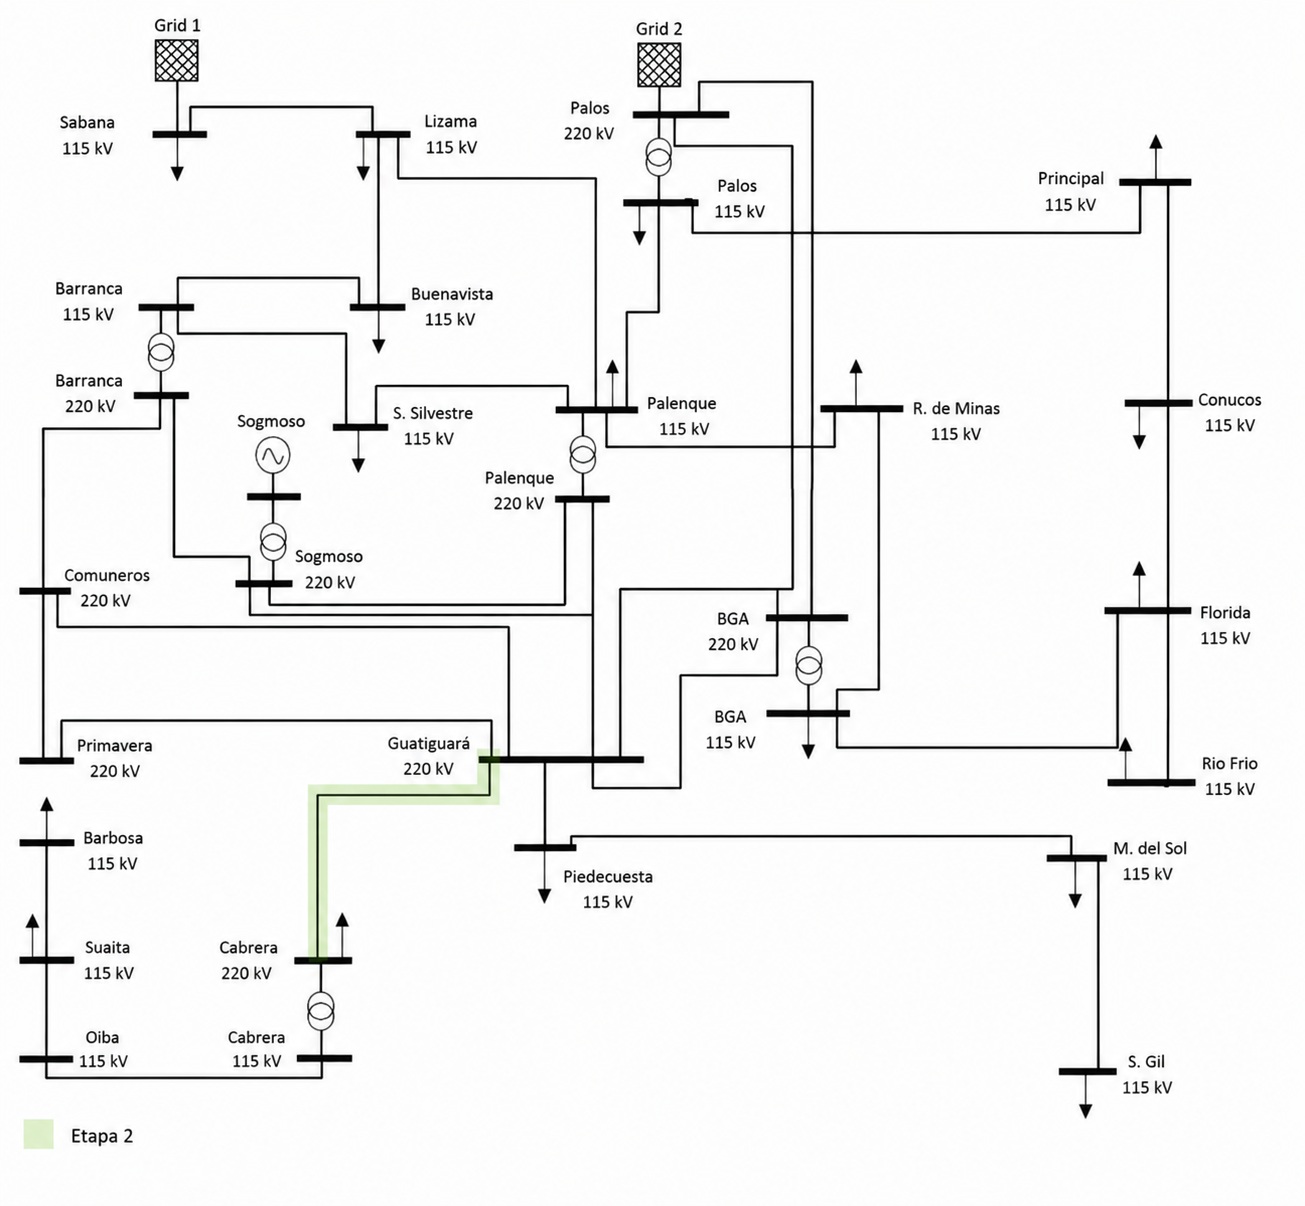
\includegraphics[width=0.65\linewidth]{etapa2.png}
    \caption{Sistema de potencia en estudio: Etapa N.° 2.}
    \label{fig:etapa2}
\end{figure}

\subsection{Ubicación geográfica}
En esta sección se presenta la ubicación geográfica de las subestaciones nuevas del proyecto. En la Tabla~\ref{tab:coordenadas_subestaciones} se indican las coordenadas de latitud y longitud correspondientes a cada una de ellas.
\begin{table}[H]
\centering
\caption{Coordenadas geográficas de las subestaciones}
\label{tab:coordenadas_subestaciones}
\begin{tabular}{|c|c|c|}
\hline
\textbf{Subestación} & \textbf{Latitud} & \textbf{Longitud} \\ \hline
Piedecuesta 115   & 6.99770 & -73.05030 \\ \hline
Mesa del Sol 115  & 6.81467 & -73.08495 \\ \hline
San Gil 115       & 6.45928 & -73.15218 \\ \hline
Cabrera 115 / 220 & 6.40877 & -73.18134 \\ \hline
Oiba 115          & 6.05306 & -73.38653 \\ \hline
Suaita 115        & 5.87971 & -73.53146 \\ \hline
Barbosa 115       & 5.63658 & -73.78651 \\ \hline
Guatiguará 220    & 6.96485 & -73.05762 \\ \hline
\end{tabular}
\end{table}
\subsection{Área de influencia}
En la Figura~\ref{fig:areainflu} se presenta el área de influencia del proyecto, delimitada mediante las zonas resaltadas en el mapa. Esta área comprende tanto la infraestructura existente como las intervenciones correspondientes a las diferentes etapas de desarrollo del proyecto. La zona identificada en color morado corresponde a la infraestructura que hace parte del área de influencia y que se encontraba previamente existente. Por su parte, el color azul representa los elementos correspondientes a la Etapa 1, mientras que el color verde identifica los elementos asociados a la Etapa 2. En conjunto, estas zonas conforman el área de influencia considerada para el desarrollo y análisis del proyecto.
\begin{figure}[H]
    \centering
    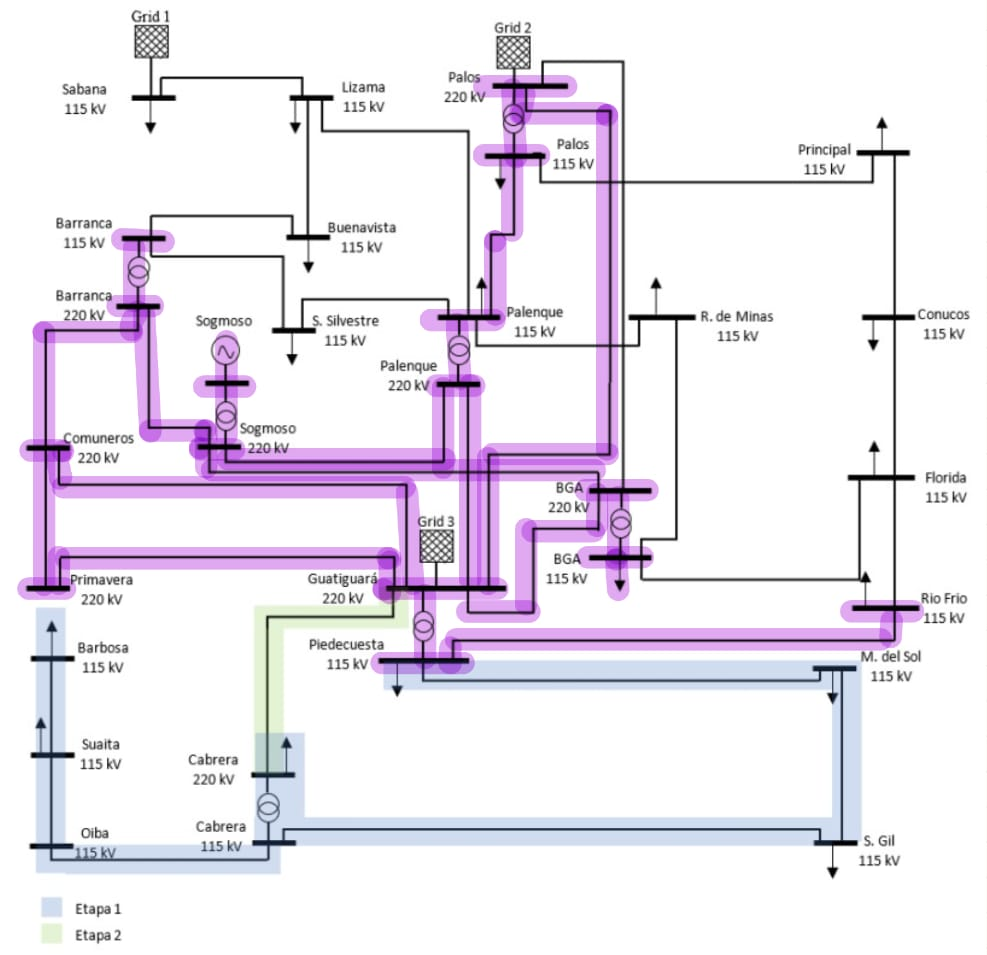
\includegraphics[width=0.8\linewidth]{areainflu.jpeg}
    \caption{Área de influencia del proyecto}
    \label{fig:areainflu}
\end{figure}

\section{Parámetros técnicos}
En esta sección se presentan los parámetros técnicos de los equipos de potencia considerados dentro del alcance del proyecto.
\subsection{Parámetros de equipos}
\subsubsection{Parámetros de líneas de transmisión}


\begin{center}
\small
\setlength{\tabcolsep}{2pt}
\renewcommand{\arraystretch}{1.15}

\begin{longtable}{|p{5.8cm}|r|r|r|r|r|r|r|r|r|}
\caption{Parámetros técnicos de líneas}
\label{tab:parametros_lineas} \\

\hline
\textbf{Línea} &
\makecell{\textbf{Long.}\\\textbf{[km]}} &
\makecell{\textbf{$R_1$}\\\textbf{[$\Omega$/km]}} &
\makecell{\textbf{$X_1$}\\\textbf{[$\Omega$/km]}} &
\makecell{\textbf{$R_0$}\\\textbf{[$\Omega$/km]}} &
\makecell{\textbf{$X_0$}\\\textbf{[$\Omega$/km]}} &
\makecell{\textbf{$B_0$*}\\\textbf{[S/km]}} &
\makecell{\textbf{$B_1$*}\\\textbf{[S/km]}} &
\makecell{\textbf{$I_{\mathrm{Nom.}}$}\\\textbf{[A]}} &
\makecell{\textbf{$I_{\mathrm{Emerg.}}$}\\\textbf{[A]}} \\
\hline
\endfirsthead

\hline
\multicolumn{10}{|c|}{\textit{Tabla \thetable{} -- continuación}} \\
\hline

\textbf{Línea} &
\makecell{\textbf{Long.}\\\textbf{[km]}} &
\makecell{\textbf{$R_1$}\\\textbf{[$\Omega$/km]}} &
\makecell{\textbf{$X_1$}\\\textbf{[$\Omega$/km]}} &
\makecell{\textbf{$R_0$}\\\textbf{[$\Omega$/km]}} &
\makecell{\textbf{$X_0$}\\\textbf{[$\Omega$/km]}} &
\makecell{\textbf{$B_0$}\textsuperscript{*}\\\textbf{[S/km]}} &
\makecell{\textbf{$B_1$}\textsuperscript{*}\\\textbf{[S/km]}} &
\makecell{\textbf{$I_{\mathrm{Nom.}}$}\\\textbf{[A]}} &
\makecell{\textbf{$I_{\mathrm{Emerg.}}$}\\\textbf{[A]}} \\
\hline
\endhead

\hline
\multicolumn{10}{|r|}{\textit{Continúa en la siguiente página}} \\
\hline
\endfoot

\hline
\endlastfoot

\hline
\endlastfoot

Barranca - Buenavista 115 kV & 12.10 & 0.1934 & 0.4132 & 0.3413 & 1.2579 & 0 & 0 & 530 & 662.5 \\
\hline
Buenavista - Lizama 115 kV & 36.50 & 0.1932 & 0.4126 & 0.3405 & 1.2562 & 0 & 0 & 530 & 662.5 \\
\hline
Lizama - Sabana 115 kV & 33.10 & 0.1622 & 0.4127 & 0.3100 & 1.2332 & 0 & 0 & 240 & 300 \\
\hline
Lizama - Palenque 115 kV & 45.60 & 0.1934 & 0.4132 & 0.3410 & 1.2575 & 0 & 0 & 530 & 662.5 \\
\hline
Palenque - S. Silvestre 115 kV & 80.20 & 0.1792 & 0.4783 & 0.8676 & 1.3173 & 0 & 0 & 480 & 600 \\
\hline
Barranca - S. Silvestre 115 kV & 8.60 & 0.1872 & 0.4919 & 0.3640 & 1.4965 & 0 & 0 & 530 & 662.5 \\
\hline
Barranca - Sogamoso 220 kV & 52.56 & 0.0797 & 0.4882 & 0.2546 & 1.3900 & 0 & 0 & 900 & 1125 \\
\hline
Barranca - Comuneros 220 kV & 10.90 & 0.0725 & 0.5349 & 0.4202 & 1.3450 & 0 & 0 & 810 & 1011.25 \\
\hline
Comuneros - Primavera 220 kV & 111.60 & 0.0705 & 0.5515 & 0.3531 & 1.5300 & 0 & 0 & 810 & 1012.5 \\
\hline
Comuneros - Guatiguará 220 kV & 95.20 & 0.0525 & 0.4749 & 0.2090 & 1.0298 & 0 & 0 & 810 & 1012.5 \\
\hline
Primavera - Guatiguará 220 kV & 162.90 & 0.0543 & 0.4767 & 0.2659 & 1.2971 & 0 & 0 & 980 & 1225 \\
\hline
Guatiguará - Palenque 220 kV & 45.00 & 0.0513 & 0.4882 & 0.2227 & 1.7271 & 0 & 0 & 1000 & 1250 \\
\hline
Palenque - Palos 115 kV & 10.70 & 0.1925 & 0.4907 & 0.3701 & 1.4935 & 0 & 0 & 530 & 662.5 \\
\hline
Palos - Guatiguará 220 kV & 30.60 & 0.0614 & 0.4837 & 0.2781 & 1.1971 & 0 & 0 & 840 & 1050 \\
\hline
Guatiguará - Bucaramanga 220 kV & 12.11 & 0.0710 & 0.5120 & 0.3939 & 1.3592 & 0 & 0 & 840 & 1050 \\
\hline
Sogamoso - Palenque 220 kV & 40.00 & 0.0512 & 0.4883 & 0.2225 & 1.7270 & 0 & 0 & 1000 & 1250 \\
\hline
Sogamoso - Bucaramanga 220 kV & 44.70 & 0.0801 & 0.4911 & 0.2559 & 1.3980 & 0 & 0 & 900 & 1125 \\
\hline
Palenque - Real de Minas 115 kV & 5.12 & 0.2129 & 0.4980 & 0.3594 & 1.3359 & 0 & 0 & 530 & 662.5 \\
\hline
Real de Minas - Bucaramanga 115 kV & 8.68 & 0.2281 & 0.4758 & 0.3975 & 1.4309 & 0 & 0 & 530 & 662.5 \\
\hline
Palos - Principal 115 kV & 4.20 & 0.1167 & 0.4500 & 0.3238 & 1.3000 & 0 & 0 & 520 & 650 \\
\hline
Principal - Conucos 115 kV & 12.74 & 0.1264 & 0.5118 & 0.3438 & 1.3854 & 0 & 0 & 520 & 650 \\
\hline
Conucos - Florida 115 kV & 11.81 & 0.1338 & 0.5368 & 0.3429 & 1.4598 & 0 & 0 & 520 & 650 \\
\hline
Florida - Rio Frio 115 kV & 3.60 & 0.1194 & 0.4778 & 0.4722 & 1.3694 & 0 & 0 & 550 & 687.5 \\
\hline
Bucaramanga - Palos 220 kV & 23.45 & 0.0789 & 0.4925 & 0.2546 & 1.5565 & 0 & 0 & 900 & 1125 \\
\hline
Florida - Bucaramanga 115 kV & 1.74 & 0.1437 & 0.5402 & 0.3218 & 1.5172 & 0 & 0 & 590 & 737.5 \\
\hline
Rio Frio - Piedecuesta 115 kV & 11.95 & 0.1364 & 0.5004 & 0.2711 & 1.0603 & 0 & 0 & 530 & 662.5 \\
\hline
Piedecuesta - Mesa del Sol 115 kV & 20.60 & 0.2126 & 0.5170 & 0.3898 & 1.6272 & 0 & 0 & 1000 & 1250 \\
\hline
San Gil- Mesa del Sol 115 kV & 40.00 & 0.2130 & 0.5170 & 0.3900 & 1.6270 & 0 & 0 & 460 & 575 \\
\hline
San Gil - Cabrera 115 kV & 6.45 & 0.2129 & 0.5171 & 0.3898 & 1.6279 & 0 & 0 & 460 & 575 \\
\hline
Cabrera - Oiba 115 kV & 45.42 & 0.1990 & 0.4833 & 0.3644 & 1.5207 & 0 & 0 & 458 & 572.5 \\
\hline
Cabrera - Guatiguará 220 kV & 63.00 & 0.0502 & 0.4740 & 0.2965 & 1.1675 & 0 & 0 & 1000 & 1250 \\
\hline
Suaita - Oiba 115 kV & 25.00 & 0.2128 & 0.5172 & 0.3900 & 1.6272 & 0 & 0 & 460 & 575 \\
\hline
Suaita - Barbosa 115 kV & 39.00 & 0.2128 & 0.5172 & 0.3900 & 1.6272 & 0 & 0 & 460 & 575 \\

\end{longtable}
\end{center}

\vspace{-0.2cm}

\begin{minipage}{0.90\textwidth}
\footnotesize
\textit{(*) Las susceptancias longitudinales de las líneas se consideran iguales a cero,
despreciando su efecto debido a la longitud relativamente corta de los tramos analizados.
}
\end{minipage}

\begin{minipage}{0.90\textwidth}
\footnotesize
\textit{(**)} La corriente de emergencia se estima como el 125\% de la corriente nominal de cada línea.
\end{minipage}

\subsubsection{Parámetros de transformadores}
\begin{table}[htbp]
  \centering
  \caption{Parámetros técnicos de transformadores de potencia}
  \label{tab:params_trafos}
  \begin{threeparttable}
    \resizebox{\textwidth}{!}{%
    \begin{tabular}{|c|c|c|c|c|c|c|}
      \hline
      \textbf{Transformador} &
      \textbf{\begin{tabular}[c]{@{}c@{}}$S_{H/L}$\\ {[MVA]}$^{(3)}$\end{tabular}} &
      \textbf{\begin{tabular}[c]{@{}c@{}}$V_{H/L}$\\ {[kV]}\end{tabular}} &
      \textbf{\begin{tabular}[c]{@{}c@{}}$Z_{HL}$\\ {[\%]}\end{tabular}} &
      \textbf{\begin{tabular}[c]{@{}c@{}}$Z_{HL}$ sec 0\\ {[\%]}$^{(2)}$\end{tabular}} &
      \textbf{\begin{tabular}[c]{@{}c@{}}Sobrecarga\\ 30 min {[\%]}\tnote{(1)}\end{tabular}} &
      \textbf{\begin{tabular}[c]{@{}c@{}}Grupo de\\ conexión$^{(4)}$\end{tabular}} \\
      \hline
      TRF1 S/E Barranca            & 4 $\times$ 90  & 220/115  & 9.4    & 8.4   &  140 & YNyn0 \\ \hline
      TRF2 S/E Palenque           & 2 $\times$ 150 & 220/115  & 16.4    & 16.4  &  140 & YNyn0 \\ \hline
      TRF3 S/E Bucaramanga        & 2 $\times$ 150 & 220/115  & 16.7    & 16.7  & 140 & YNyn0 \\ \hline
      TRF4 S/E Guatiguará--Piedecuesta & 1 $\times$ 150 & 220/115 & 16.6    & 16.6  & 140 & YNyn0 \\ \hline
      TRF5 S/E Cabrera            & 2 $\times$ 150 & 220/115  & 15.0    & 15.0  &  140 & YNyn0 \\ \hline
      TRF6 S/E Palos              & 1 $\times$ 150 & 220/115  & 16.3    & 16.3  &  140 & YNyn0 \\ \hline
      TRF7 Central Sogamoso       & 3 $\times$ 324 & 220/16.5 & 12.34   & 12.34 & 140 & YNd11 \\ \hline
    \end{tabular}%
    }
  \end{threeparttable}
\end{table}

\begin{minipage}{0.90\textwidth}
\footnotesize
\textit{(1) Sobrecarga 30 min: 140\,\%. Valor estimado según IEC~60076-7 (Anexo K), refrigeración ONAF, $K_1 = 0{,}8$, $\theta_a = 30\ ^\circ$C, límite de punto caliente de emergencia 140\,$^\circ$C.
}
\end{minipage}


\subsubsection{Parámetros de generadores}

\begin{center}

\textbf{Cuadro 4: Parámetros técnicos de los generadores}

\vspace{2mm}

\scriptsize
\renewcommand{\arraystretch}{1.1}

\begin{tabular}{|c|c|p{6.0cm}|c|}
\hline

\textbf{Planta} &
\textbf{Unidad de} &
\multicolumn{1}{c|}{\textbf{Parámetro}} &
\textbf{Valor} \\

&
\textbf{generación} &
&
\\
\hline

\multirow{9}{*}{\centering Sogamoso}
&
\multirow{3}{*}{\centering U1}
& Potencia nominal [MVA] & 324 \\ \cline{3-4}
& & Tensión nominal [kV] & 16,5 \\ \cline{3-4}
& & Corriente nominal [A] & 11\,338 \\ \cline{2-4}

&
\multirow{3}{*}{\centering U2}
& Potencia nominal [MVA] & 324 \\ \cline{3-4}
& & Tensión nominal [kV] & 16,5 \\ \cline{3-4}
& & Corriente nominal [A] & 11\,338 \\ \cline{2-4}

&
\multirow{3}{*}{\centering U3}
& Potencia nominal [MVA] & 324 \\ \cline{3-4}
& & Tensión nominal [kV] & 16,5 \\ \cline{3-4}
& & Corriente nominal [A] & 11\,338 \\ \hline

\end{tabular}

\vspace{3mm}

\begin{minipage}{0.90\textwidth}
\footnotesize
\textit{Nota: Para este EACP de líneas, conforme a los Lineamientos del CNO, únicamente se requieren los datos de potencia, tensión y corriente nominal de los generadores ubicados en el área de influencia.}
\end{minipage}

\end{center}
\section{Estudio de flujo y cortocircuito}

\subsection{Análisis de flujo}

\textbf{Análisis de tensiones de barra.}
Para evaluar el comportamiento del sistema ante la incorporación del proyecto, se analizaron las tensiones de las barras de las subestaciones para los escenarios de demanda mínima, base y máxima. Se consideró la Etapa 0 como condición de referencia, correspondiente al sistema sin la incorporación del proyecto, mientras que las Etapas 1 y 2 representan su integración progresiva al SIN.



Resultados de tensiones en las barras en la etapa 0:

\begin{figure}[H]
    \centering
    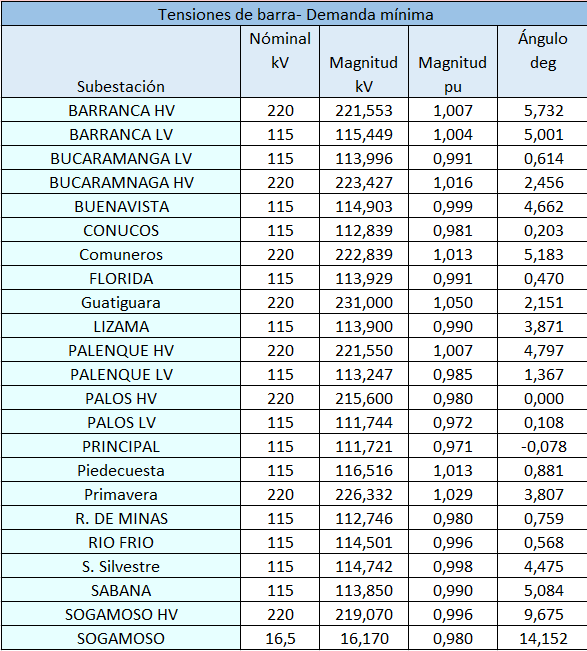
\includegraphics[width=0.6\linewidth]{VminE0.png}
    \caption{Tensión de barra por subestación - DEMANDA MÍNIMA ETAPA 0}
    \label{fig:VminE0}
\end{figure}

\begin{figure}[H]
    \centering
    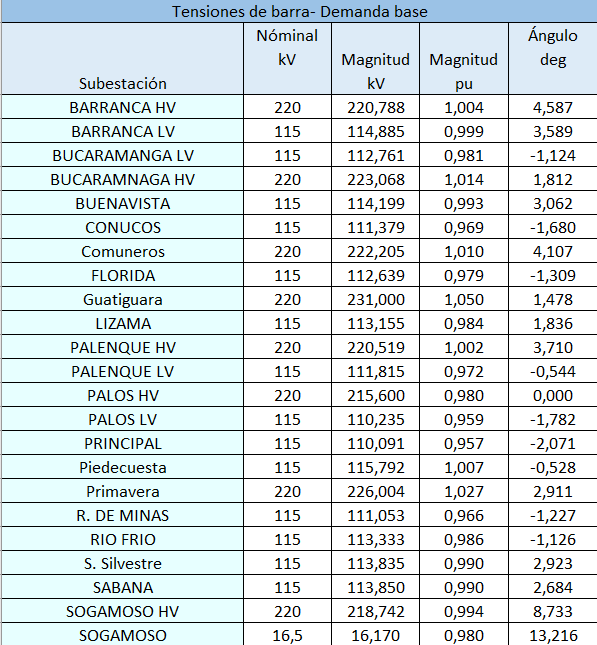
\includegraphics[width=0.6\linewidth]{VbasE0.png}
    \caption{Tensión de barra por subestación - DEMANDA BASE ETAPA 0}
    \label{fig:VbasE0}
\end{figure}

\begin{figure}[H]
    \centering
    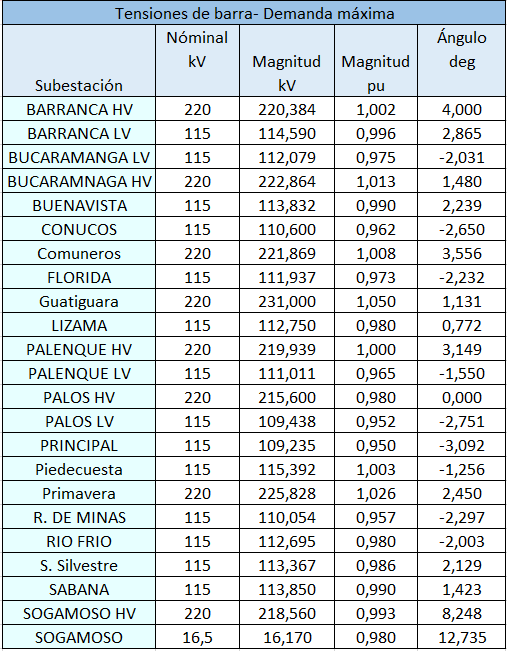
\includegraphics[width=0.6\linewidth]{VmaxE0.png}
    \caption{Tensión de barra por subestación - DEMANDA MÁXIMA ETAPA 0}
    \label{fig:VmaxE0}
\end{figure}


Resultados de tensiones en las barras en la etapa 1:
\begin{figure}[H]
    \centering
    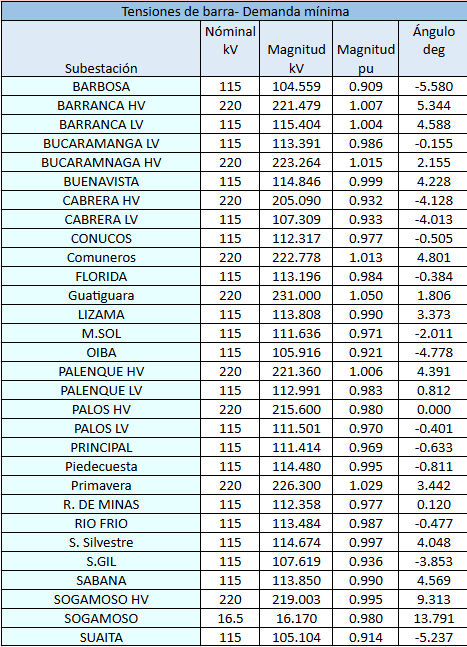
\includegraphics[width=0.6\linewidth]{VminE1.png}
    \caption{Tensión de barra por subestación - DEMANDA MÍNIMA ETAPA 1}
    \label{fig:VminE1}
\end{figure}

\begin{figure}[H]
    \centering
    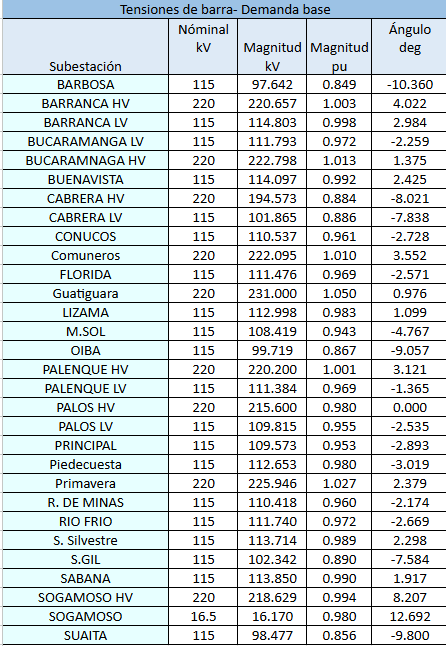
\includegraphics[width=0.6\linewidth]{VbasE1.png}
    \caption{Tensión de barra por subestación - DEMANDA BASE ETAPA 1}
    \label{fig:VbasE1}
\end{figure}

\begin{figure}[H]
    \centering
    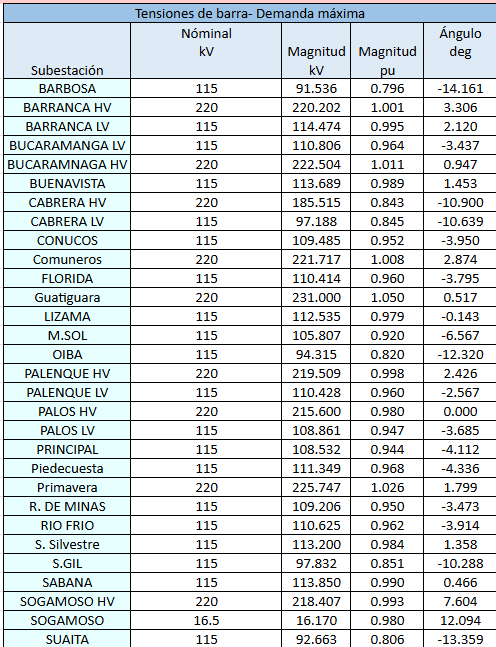
\includegraphics[width=0.6\linewidth]{VmaxE1.png}
    \caption{Tensión de barra por subestación - DEMANDA MÁXIMA ETAPA 1}
    \label{fig:VmaxE1}
\end{figure}


Resultados de tensiones en las barras en la etapa 2:

\begin{figure}[H]
    \centering
    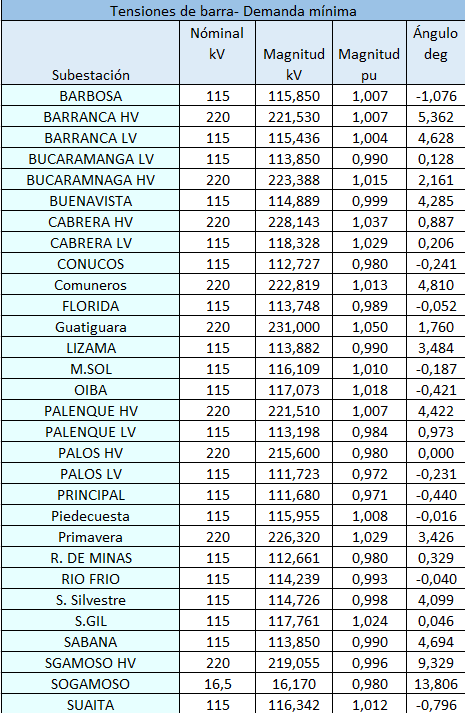
\includegraphics[width=0.6\linewidth]{VminE2.png}
    \caption{Tensión de barra por subestación - DEMANDA MÍNIMA ETAPA 2}
    \label{fig:VminE2}
\end{figure}

\begin{figure}[H]
    \centering
    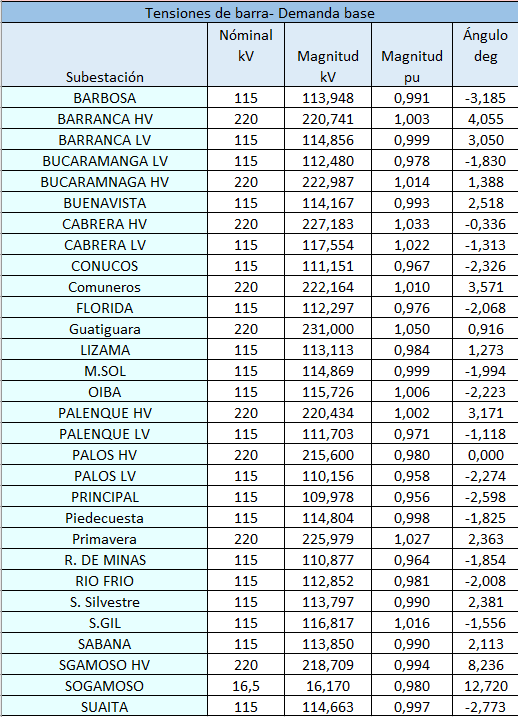
\includegraphics[width=0.6\linewidth]{VbasE2.png}
    \caption{Tensión de barra por subestación - DEMANDA BASE ETAPA 2}
    \label{fig:VbasE2}
\end{figure}

\begin{figure}[H]
    \centering
    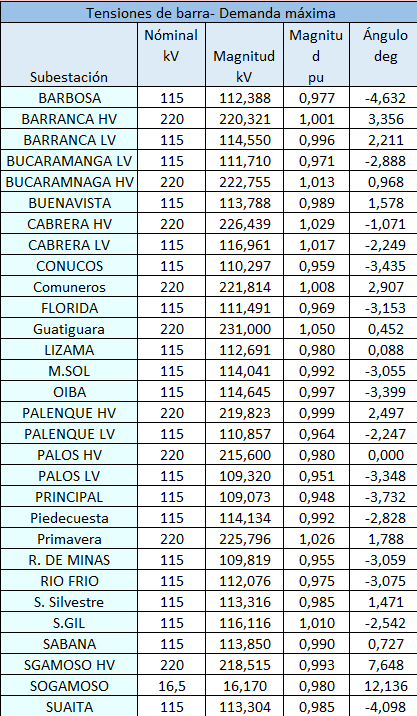
\includegraphics[width=0.6\linewidth]{VmaxE2.png}
    \caption{Tensión de barra por subestación - DEMANDA MÁXIMA ETAPA 2}
    \label{fig:VmaxE2}
\end{figure}

Con el fin de complementar los resultados presentados en las tablas anteriores y facilitar la identificación de las variaciones de tensión entre los diferentes escenarios de demanda, se presentan los gráficos de rango de tensión para cada etapa del proyecto. La Figura~\ref{fig:rango_tension} presenta la simbología empleada para la interpretación de estos gráficos, en la cual se indica el significado del punto, el rango de variación y la condición de la tensión respecto a los límites establecidos.

\begin{figure}[H]
    \centering
    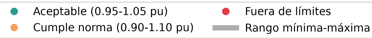
\includegraphics[width=0.8\linewidth]{rango.png}
    \caption{Rango de tensión por demandas}
    \label{fig:rango_tension}
\end{figure}

\begin{figure}[H]
    \centering
    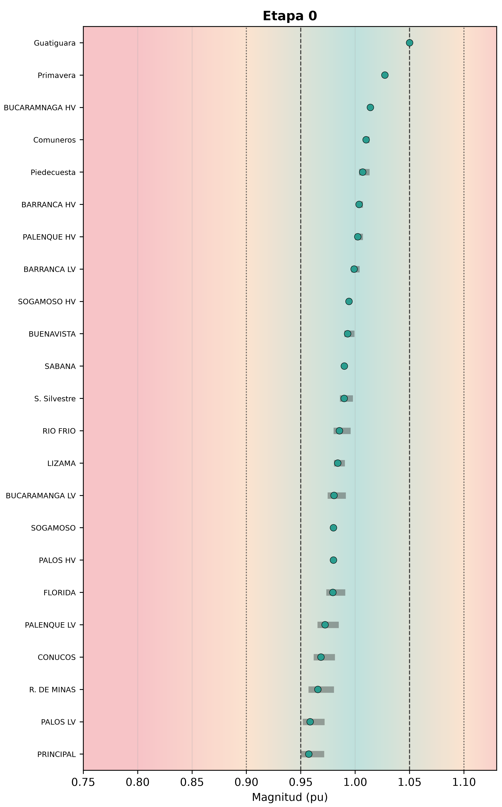
\includegraphics[width=0.65\linewidth]{vminmaxE0.png}
    \caption{Rango de tensión por demandas -ETAPA 0}
    \label{fig:vminmaxE0}
\end{figure}

\begin{figure}[H]
    \centering
    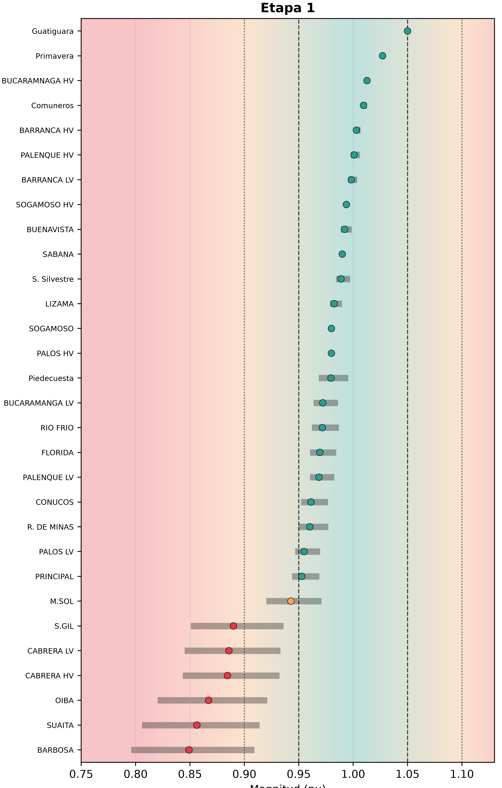
\includegraphics[width=0.65\linewidth]{vminmaxE1.png}
    \caption{Rango de tensión por demandas -ETAPA 1}
    \label{fig:vminmaxE1}
\end{figure}

\begin{figure}[H]
    \centering
    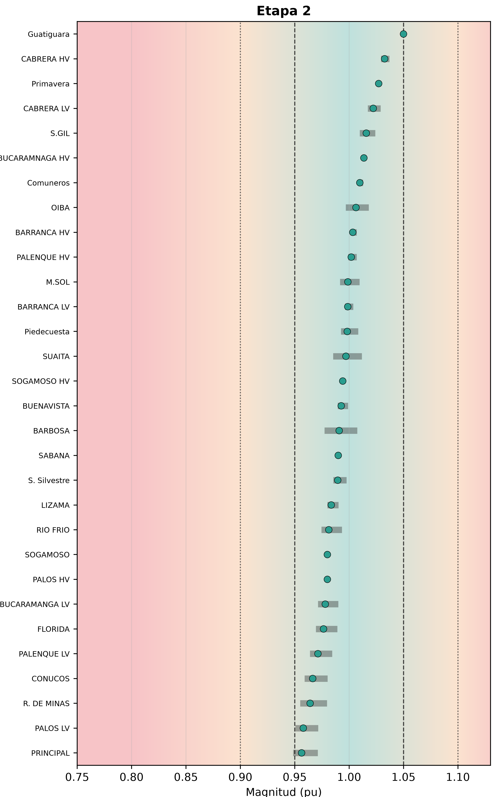
\includegraphics[width=0.65\linewidth]{vminmaxE2.png}
    \caption{Rango de tensión por demandas -ETAPA 2}
    \label{fig:vminmaxE2}
\end{figure}

En la Etapa 0, correspondiente a la condición del sistema sin la incorporación del proyecto, las tensiones de las barras analizadas se encuentran dentro del rango de 0,95 a 1,05 pu, evidenciando un comportamiento adecuado del sistema. Con la implementación de la Etapa 1, se presentan variaciones en el perfil de tensión, identificándose valores por fuera de los límites admisibles en las subestaciones de Barbosa, Suaita, Oiba, Cabrera HV, Cabrera LV y San Gil. Por su parte, Mesa del Sol permanece dentro del rango admisible, mientras que las demás barras mantienen tensiones entre 0,95 y 1,05 pu. Finalmente, con la incorporación de la Etapa 2, todas las tensiones retornan al intervalo de 0,95 a 1,05 pu, evidenciando una mejora en el perfil de tensión y el cumplimiento de los límites establecidos por la normativa aplicable.


Como complemento al análisis anterior, se presenta el diagrama de calor de las tensiones de barra para la demanda base, con el propósito de visualizar de manera conjunta la magnitud de tensión en las diferentes subestaciones y su evolución con la incorporación progresiva del proyecto. La Figura~\ref{fig:tensionbase} permite comparar el perfil de tensión entre las Etapas 0, 1 y 2, facilitando la identificación de las barras que presentan mayores variaciones respecto a la condición inicial del sistema.

\begin{figure}[H]
    \centering
    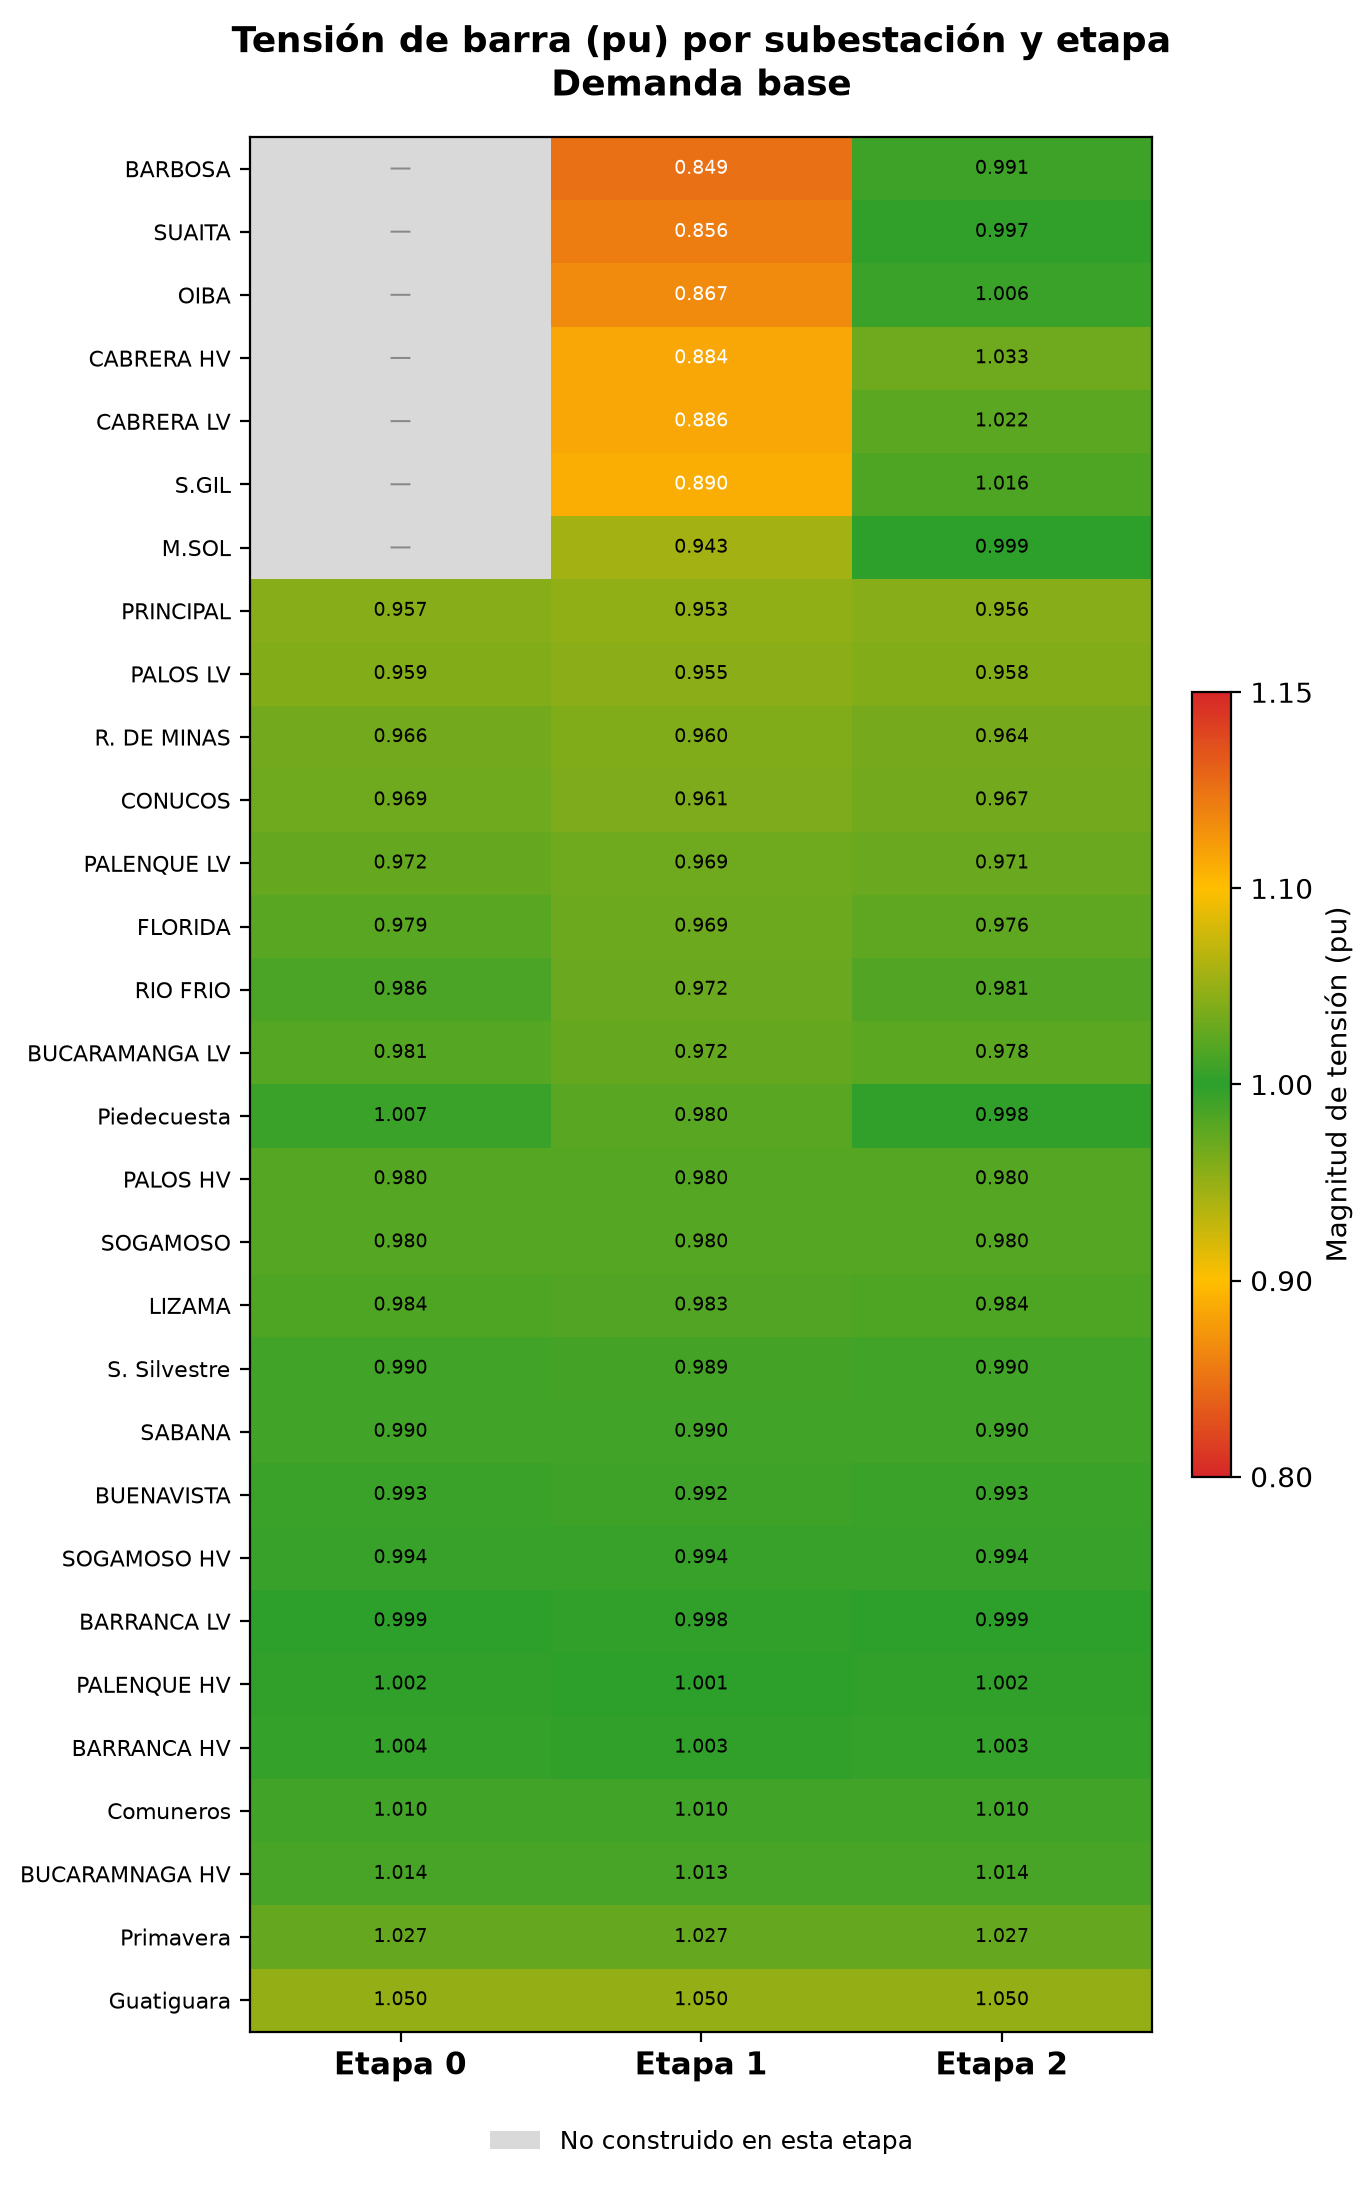
\includegraphics[width=0.8\linewidth]{TENSIONBASE.png}
    \caption{Tensión de barra por subestación y etapa - DEMANDA BASE}
    \label{fig:tensionbase}
\end{figure}

Como resultado del estudio de flujo de carga desarrollado para la Etapa 1, se identificaron problemas de regulación de tensión evidenciados por condiciones de subtensión en varias barras del área de influencia. Específicamente, las subestaciones Barbosa, Suaita, Oiba, Cabrera (tanto en 115 kV como en el nivel secundario) y San Gil registraron niveles de tensión por debajo del límite operativo de 0,90 pu, siendo la barra de Barbosa 115 kV la que presentó la condición más desfavorable, con un valor de 0,849 pu.

Ante este escenario de déficit de tensión, se implementó como medida de solución la incorporación de un banco de capacitores tipo \textit{shunt}, ubicado en la subestación Barbosa 115 kV. Mediante simulaciones iterativas en DIgSILENT PowerFactory, se determinó que se requería una compensación mínima de 17 MVAr para restituir los perfiles de tensión de todos los nodos afectados dentro de los rangos permitidos. Con base en este resultado, se seleccionó un equipo comercial de 22,5 MVAr a 115 kV, del fabricante EPRECSA, cuya capacidad cubre el requerimiento mínimo obtenido mediante simulación y permite solucionar los problemas de regulación identificados en esta etapa.

\begin{center}

\textbf{Cuadro 5: Características técnicas del banco de capacitores seleccionado}

\vspace{2mm}

\normalsize
\renewcommand{\arraystretch}{2.5}

\begin{tabular}{|l|c|}
\hline
\textbf{Característica} & \textbf{Valor} \\ \hline
Fabricante & EPRECSA \\ \hline
Referencia & BCM-115-22.50-13.28 \\ \hline
Tensión nominal & 115 kV \\ \hline
Potencia reactiva nominal & 22,5 MVAr \\ \hline
\end{tabular}

\end{center}


Teniendo en cuenta lo anterior, a continuación se muestran los resultados de tensiones en las barras en la etapa 1 con compensación:

\begin{figure}[H]
    \centering
    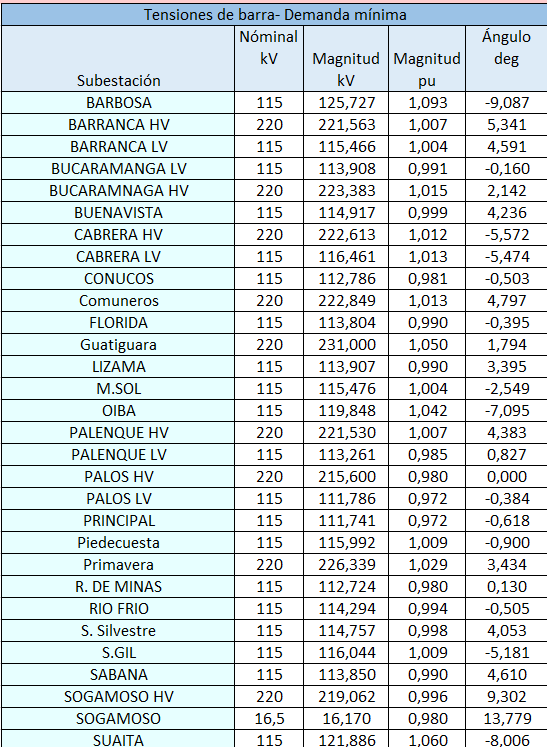
\includegraphics[width=0.6\linewidth]{VminE1c.png}
    \caption{Tensión de barra por subestación - DEMANDA MÍNIMA ETAPA 1 con compensación}
    \label{fig:VminE1c}
\end{figure}

\begin{figure}[H]
    \centering
    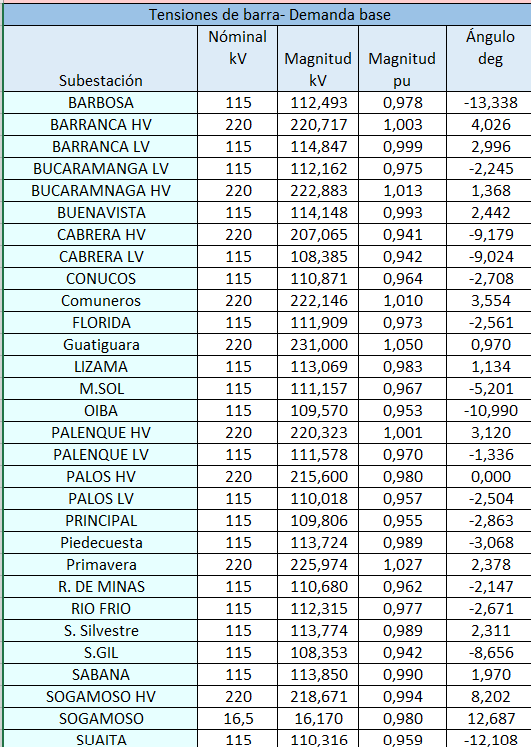
\includegraphics[width=0.6\linewidth]{VbasE1c.png}
    \caption{Tensión de barra por subestación - DEMANDA BASE ETAPA 1 con compensación}
    \label{fig:VbasE1c}
\end{figure}

\begin{figure}[H]
    \centering
    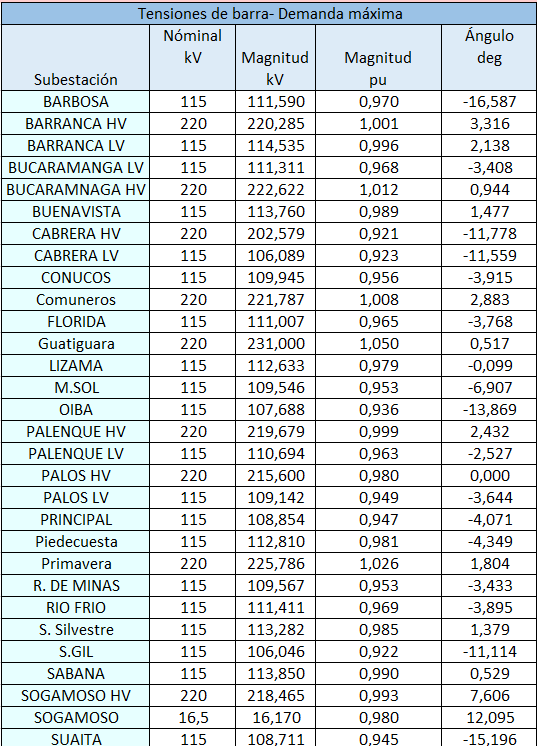
\includegraphics[width=0.6\linewidth]{VmaxE1c.png}
    \caption{Tensión de barra por subestación - DEMANDA MÁXIMA ETAPA 1 con compensación}
    \label{fig:VmaxE1c}
\end{figure}
Como se observa en la Figura~\ref{fig:VmaxE1c}, con ayuda del banco de capacitores, ya no se presentan problemas de regulación de tensión
\begin{figure}[H]
    \centering
    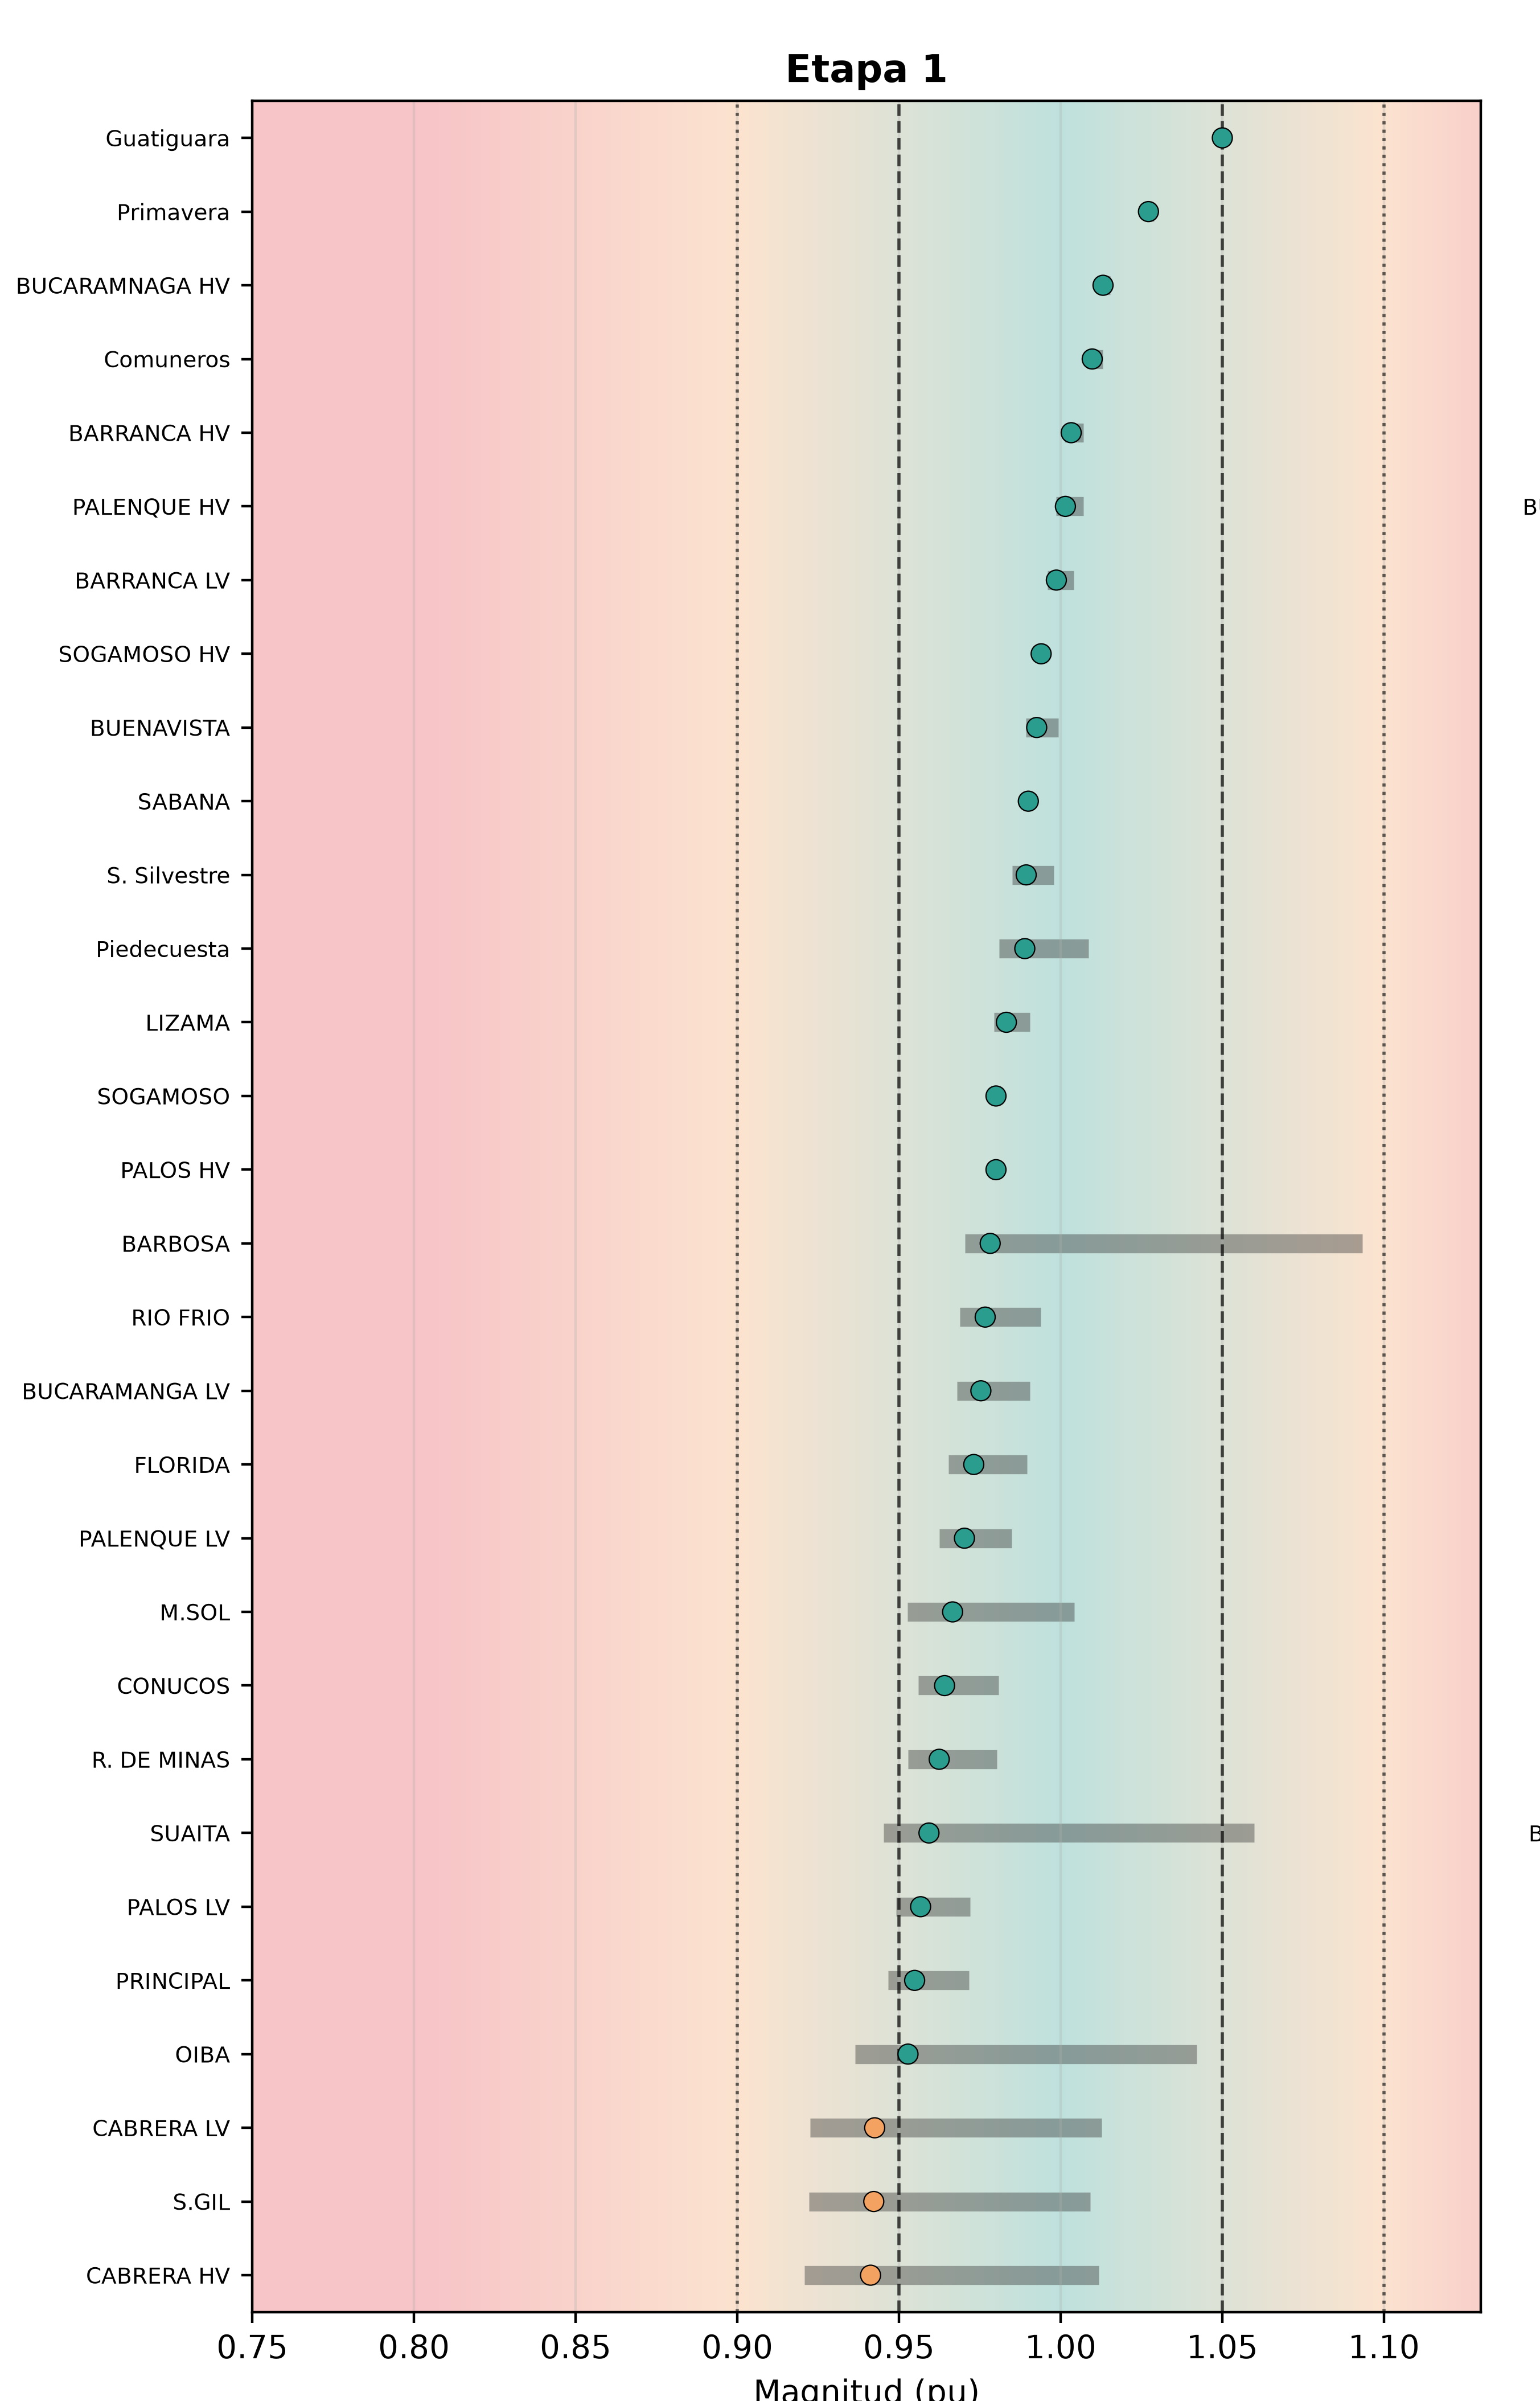
\includegraphics[width=0.8\linewidth]{cargE1cgraf.png}
    \caption{Cargabilidad elementos por demandas - ETAPA 1 con compensación}
    \label{fig:cargE1cgraf}
\end{figure}



\textbf{Análisis de cargabilidad de los elementos.} Como complemento al análisis del comportamiento de las tensiones, se evaluó la cargabilidad de las líneas de transmisión y transformadores para los escenarios de demanda mínima, base y máxima, considerando las diferentes etapas de incorporación del proyecto. Este análisis permite identificar el nivel de utilización de cada elemento y determinar la posible presencia de condiciones de sobrecarga. Los resultados obtenidos para cada escenario y etapa se presentan en las tablas siguientes, donde se relaciona la cargabilidad de los elementos con respecto a su capacidad nominal.

\begin{figure}[H]
    \centering
    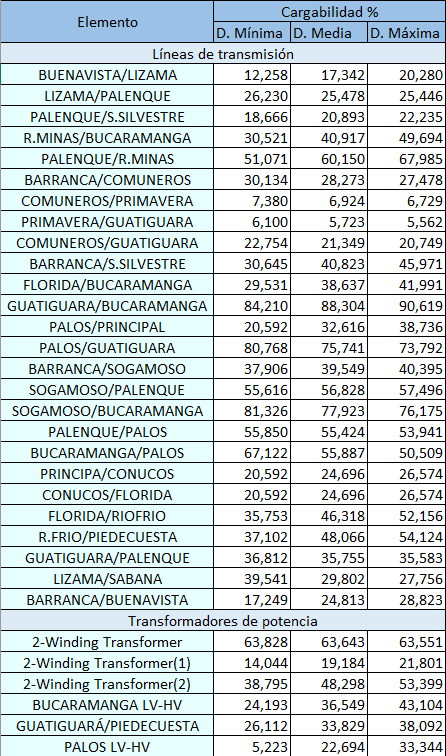
\includegraphics[width=0.6\linewidth]{cargE0.png}
    \caption{Cargabilidad elementos - ETAPA 0}
    \label{fig:cargE0}
\end{figure}

\begin{figure}[H]
    \centering
    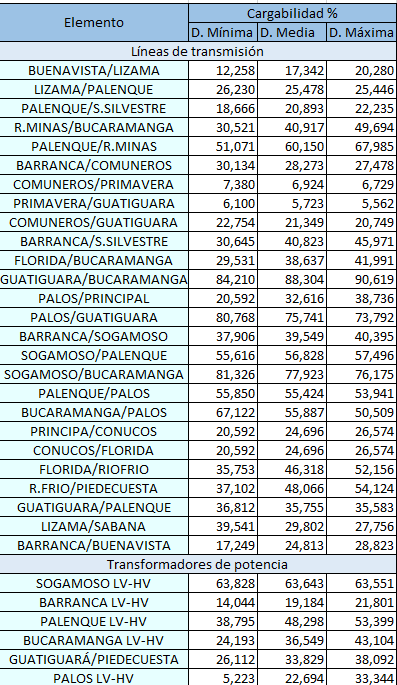
\includegraphics[width=0.6\linewidth]{cargE1.png}
    \caption{Cargabilidad elementos - ETAPA 1 sin compensación}
    \label{fig:cargE1_sin_comp}
\end{figure}

\begin{figure}[H]
    \centering
    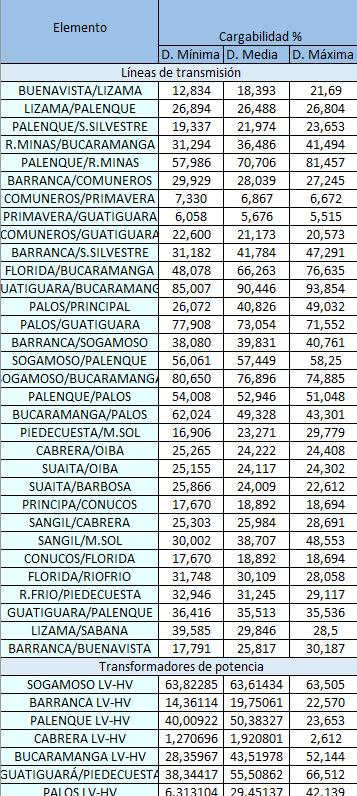
\includegraphics[width=0.58\linewidth]{cargE1c.png}
    \caption{Cargabilidad elementos - ETAPA 1 con compensación}
    \label{fig:cargE1c}
\end{figure}

\begin{figure}[H]
    \centering
    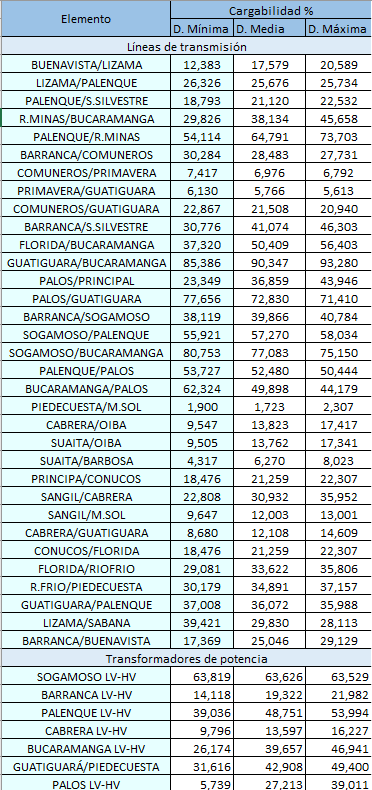
\includegraphics[width=0.6\linewidth]{cargE2.png}
    \caption{Cargabilidad elementos - ETAPA 2}
    \label{fig:cargE2}
\end{figure}

Para una mejor visualización de los resultados, se hizo uso de los siguientes gráficos, en ellos podemos hacer la comparación de la cargabilidad de los elementos por cada etapa del proyecto. Para la comprensión de las figuras se tiene en cuenta lo siguiente:

\begin{figure}[H]
    \centering
    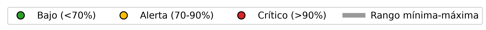
\includegraphics[width=1\linewidth]{rangocarg.png}
    \caption{Rango cargabilidad elementos }
    \label{fig:rangocarg}
\end{figure}

\begin{figure}[H]
    \centering
    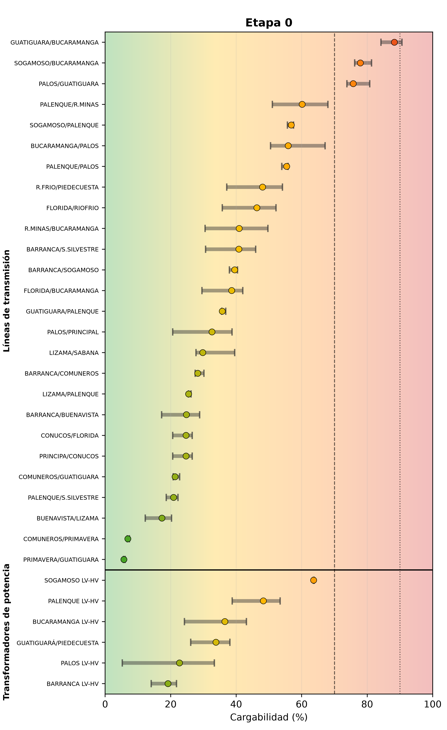
\includegraphics[width=0.7\linewidth]{cargmmE0.png}
    \caption{Rango de cargabilidad elementos - ETAPA E0}
    \label{fig:cargmmE0}
\end{figure}

\begin{figure}[H]
    \centering
    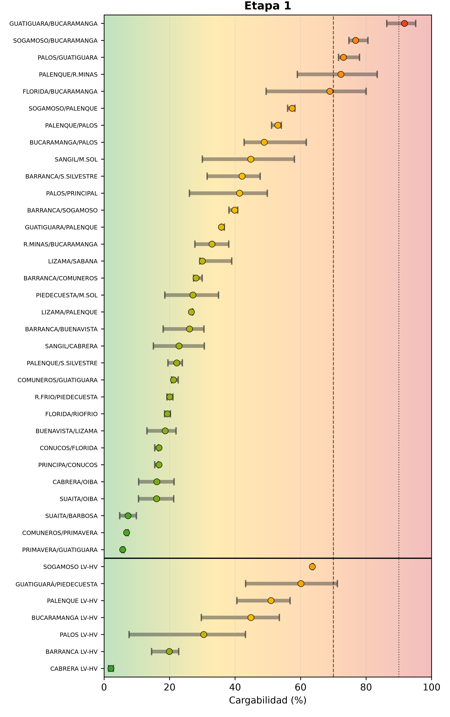
\includegraphics[width=0.7\linewidth]{cargmmE1.png}
    \caption{Rango de cargabilidad elementos - ETAPA E1}
    \label{fig:cargmmE1}
\end{figure}

\begin{figure}[H]
    \centering
    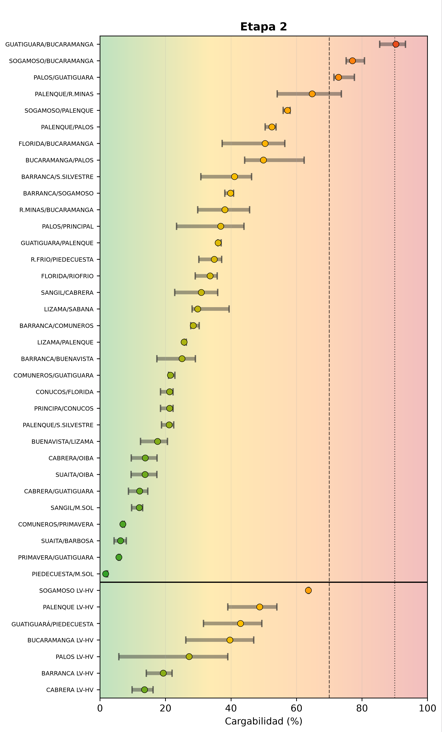
\includegraphics[width=0.7\linewidth]{cargmmE2.png}
    \caption{Rango de cargabilidad elementos - ETAPA E2}
    \label{fig:cargmmE2}
\end{figure}

\begin{figure}[H]
    \centering
    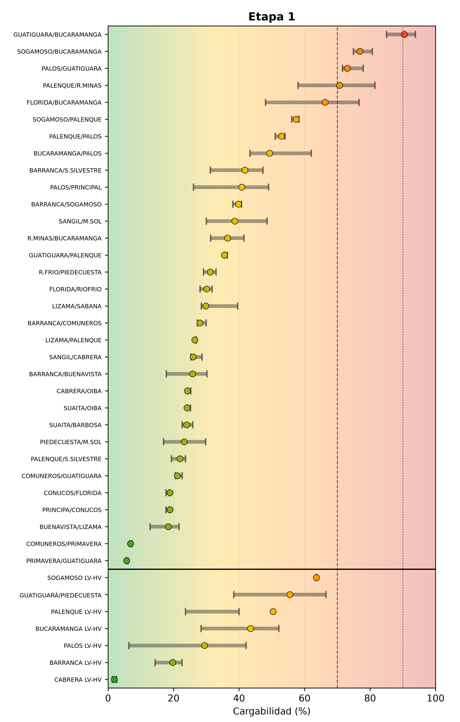
\includegraphics[width=0.8\linewidth]{cargcompE1.png}
    \caption{Rango de tensión por demandas - ETAPA 1 con compensación}
    \label{fig:cargcompE1}
\end{figure}

Como se observa, ningún elemento del sistema sobrepasó el 100\% de cargabilidad. La línea entre Guatiguará y Bucaramanga es la que presenta mayor cargabilidad, sin embargo, sigue estando dentro de los límites admisibles.



\subsection{Resultados de cortocircuito}

En las Tablas~\ref{tab:cc_demanda_minima_E0_E1} y~\ref{tab:cc_demanda_maxima_E0_E1} se presentan los resultados del análisis de cortocircuito para las condiciones de demanda mínima  y máxima, comparando la Etapa 0 con la Etapa 1 del proyecto, esta última considerando la incorporación de los elementos de compensación previstos. Esta comparación permite evaluar la variación de las corrientes de cortocircuito producida por la implementación del proyecto y los equipos de compensación, identificando los posibles cambios en los niveles de cortocircuito de las barras analizadas.

\begin{table}[H]
\centering
\caption{Resultados de cortocircuito en demanda mínima - E0 E1 compensada}
\label{tab:cc_demanda_minima_E0_E1}
\resizebox{\linewidth}{!}{%
\renewcommand{\arraystretch}{1.2}
\begin{tabular}{|l|c|c|c|c|c|c|c|c|c|c|c|c|c|c|c|c|c|c|}
\hline
\multirow{3}{*}{\textbf{Barra}} & \multicolumn{6}{c|}{\textbf{Icc demanda mínima sin proyecto [kA]}} & \multicolumn{6}{c|}{\textbf{Icc demanda mínima con proyecto [kA]}} & \multicolumn{6}{c|}{\textbf{Variación Icc demanda mínima con/sin proyecto [\%]}} \\
\cline{2-19}
 & \multicolumn{2}{c|}{1F} & \multicolumn{2}{c|}{2FT} & \multicolumn{1}{c|}{2F} & \multicolumn{1}{c|}{3F} & \multicolumn{2}{c|}{1F} & \multicolumn{2}{c|}{2FT} & \multicolumn{1}{c|}{2F} & \multicolumn{1}{c|}{3F} & \multicolumn{2}{c|}{1F} & \multicolumn{2}{c|}{2FT} & \multicolumn{1}{c|}{2F} & \multicolumn{1}{c|}{3F} \\
\cline{2-19}
 & Ikss & 3I0 & Ikss & 3I0 & Ikss & Ikss & Ikss & 3I0 & Ikss & 3I0 & Ikss & Ikss & Ikss & 3I0 & Ikss & 3I0 & Ikss & Ikss \\
\hline
BARRANCA HV & 5.45 & 5.45 & 6.86 & 4.30 & 6.42 & 7.40 & 5.46 & 5.46 & 6.86 & 4.30 & 6.42 & 7.40 & 0.02 & 0.02 & 0.05 & 0.00 & 0.05 & 0.05 \\
\hline
BARRANCA LV & 7.97 & 7.97 & 9.28 & 6.65 & 8.58 & 9.88 & 7.97 & 7.97 & 9.28 & 6.65 & 8.58 & 9.89 & 0.02 & 0.02 & 0.04 & 0.00 & 0.04 & 0.04 \\
\hline
BUCARAMANGA LV & 13.20 & 13.20 & 14.63 & 11.89 & 12.77 & 14.72 & 13.38 & 13.38 & 14.93 & 12.00 & 13.03 & 15.01 & 1.41 & 1.41 & 2.02 & 0.93 & 1.98 & 1.98 \\
\hline
BUCARAMNAGA HV & 16.58 & 16.58 & 19.95 & 14.09 & 17.06 & 19.62 & 16.62 & 16.62 & 20.00 & 14.12 & 17.11 & 19.68 & 0.22 & 0.22 & 0.27 & 0.17 & 0.30 & 0.30 \\
\hline
BUENAVISTA & 4.83 & 4.83 & 6.24 & 3.76 & 5.82 & 6.72 & 4.83 & 4.83 & 6.25 & 3.76 & 5.83 & 6.72 & 0.01 & 0.01 & 0.03 & -0.00 & 0.03 & 0.03 \\
\hline
CONUCOS & 6.40 & 6.40 & 7.97 & 5.10 & 7.42 & 8.56 & 6.43 & 6.43 & 8.05 & 5.11 & 7.49 & 8.64 & 0.54 & 0.54 & 0.97 & 0.29 & 0.93 & 0.93 \\
\hline
Comuneros & 5.17 & 5.17 & 6.52 & 4.06 & 6.13 & 7.06 & 5.17 & 5.17 & 6.52 & 4.06 & 6.13 & 7.06 & 0.02 & 0.02 & 0.04 & 0.01 & 0.05 & 0.05 \\
\hline
FLORIDA & 11.73 & 11.73 & 13.28 & 10.27 & 11.80 & 13.60 & 11.95 & 11.95 & 13.62 & 10.40 & 12.10 & 13.95 & 1.84 & 1.84 & 2.60 & 1.27 & 2.57 & 2.56 \\
\hline
Guatiguara & 39.87 & 39.87 & 44.98 & 57.89 & 25.69 & 29.53 & 40.04 & 40.04 & 45.16 & 58.08 & 25.81 & 29.67 & 0.41 & 0.41 & 0.39 & 0.32 & 0.46 & 0.46 \\
\hline
LIZAMA & 4.09 & 4.09 & 5.33 & 3.18 & 4.93 & 5.69 & 4.09 & 4.09 & 5.34 & 3.18 & 4.94 & 5.70 & 0.02 & 0.02 & 0.05 & 0.00 & 0.05 & 0.04 \\
\hline
PALENQUE HV & 7.89 & 7.89 & 10.23 & 6.16 & 9.41 & 10.82 & 7.90 & 7.90 & 10.24 & 6.17 & 9.42 & 10.84 & 0.09 & 0.09 & 0.14 & 0.05 & 0.15 & 0.16 \\
\hline
PALENQUE LV & 12.25 & 12.25 & 14.28 & 10.39 & 12.85 & 14.81 & 12.29 & 12.29 & 14.36 & 10.41 & 12.92 & 14.88 & 0.31 & 0.31 & 0.56 & 0.16 & 0.51 & 0.51 \\
\hline
PALOS HV & 13.34 & 13.34 & 15.66 & 11.48 & 13.62 & 15.68 & 13.36 & 13.36 & 15.68 & 11.49 & 13.64 & 15.71 & 0.12 & 0.12 & 0.15 & 0.07 & 0.18 & 0.18 \\
\hline
PALOS LV & 9.43 & 9.43 & 10.89 & 8.10 & 9.70 & 11.19 & 9.46 & 9.46 & 10.95 & 8.12 & 9.75 & 11.24 & 0.31 & 0.31 & 0.52 & 0.17 & 0.49 & 0.49 \\
\hline
PRINCIPAL & 7.53 & 7.53 & 9.12 & 6.17 & 8.34 & 9.62 & 7.56 & 7.56 & 9.17 & 6.18 & 8.38 & 9.67 & 0.31 & 0.31 & 0.56 & 0.16 & 0.53 & 0.53 \\
\hline
Piedecuesta & 8.09 & 8.09 & 8.85 & 7.41 & 7.68 & 8.86 & 8.90 & 8.90 & 9.90 & 8.03 & 8.61 & 9.92 & 10.11 & 10.11 & 11.90 & 8.48 & 12.01 & 11.99 \\
\hline
Primavera & 2.03 & 2.03 & 2.79 & 1.51 & 2.70 & 3.12 & 2.03 & 2.03 & 2.79 & 1.51 & 2.70 & 3.12 & 0.01 & 0.01 & 0.01 & 0.00 & 0.02 & 0.02 \\
\hline
R. DE MINAS & 10.01 & 10.01 & 11.99 & 8.27 & 10.91 & 12.57 & 10.05 & 10.05 & 12.09 & 8.29 & 10.99 & 12.67 & 0.45 & 0.45 & 0.82 & 0.24 & 0.75 & 0.75 \\
\hline
RIO FRIO & 9.36 & 9.36 & 10.83 & 7.95 & 9.83 & 11.33 & 9.64 & 9.64 & 11.26 & 8.13 & 10.21 & 11.77 & 2.92 & 2.92 & 3.96 & 2.22 & 3.90 & 3.90 \\
\hline
S. Silvestre & 4.83 & 4.83 & 6.19 & 3.75 & 5.87 & 6.77 & 4.83 & 4.83 & 6.19 & 3.75 & 5.87 & 6.77 & 0.01 & 0.01 & 0.03 & -0.00 & 0.03 & 0.03 \\
\hline
SABANA & 3.14 & 3.14 & 3.62 & 2.69 & 3.25 & 3.75 & 3.14 & 3.14 & 3.62 & 2.69 & 3.25 & 3.75 & 0.01 & 0.01 & 0.03 & 0.01 & 0.02 & 0.02 \\
\hline
SGAMOSO HV & 18.10 & 18.10 & 18.38 & 20.65 & 13.88 & 15.97 & 18.12 & 18.12 & 18.40 & 20.66 & 13.89 & 15.98 & 0.07 & 0.07 & 0.08 & 0.04 & 0.10 & 0.10 \\
\hline
SOGAMOSO & 242.09 & 242.09 & 257.36 & 241.98 & 210.89 & 244.18 & 242.16 & 242.16 & 257.45 & 242.02 & 210.99 & 244.30 & 0.03 & 0.03 & 0.04 & 0.02 & 0.05 & 0.05 \\
\hline
BARBOSA & - & - & - & - & - & - & 0.61 & 0.61 & 0.88 & 0.45 & 0.83 & 0.96 & - & - & - & - & - & - \\
\hline
CABRERA HV & - & - & - & - & - & - & 3.26 & 3.26 & 4.19 & 2.52 & 3.99 & 4.61 & - & - & - & - & - & - \\
\hline
CABRERA LV & - & - & - & - & - & - & 4.55 & 4.55 & 5.37 & 3.75 & 5.03 & 5.80 & - & - & - & - & - & - \\
\hline
M.SOL & - & - & - & - & - & - & 3.53 & 3.53 & 4.72 & 2.70 & 4.39 & 5.07 & - & - & - & - & - & - \\
\hline
OIBA & - & - & - & - & - & - & 1.27 & 1.27 & 1.77 & 0.95 & 1.68 & 1.94 & - & - & - & - & - & - \\
\hline
S.GIL & - & - & - & - & - & - & 3.78 & 3.78 & 4.73 & 3.00 & 4.44 & 5.13 & - & - & - & - & - & - \\
\hline
SUAITA & - & - & - & - & - & - & 0.90 & 0.90 & 1.27 & 0.66 & 1.20 & 1.39 & - & - & - & - & - & - \\
\hline
\end{tabular}%
}
\end{table}

\begin{table}[H]
\centering
\caption{Resultados de cortocircuito en demanda máxima - E0 E1 compensada}
\label{tab:cc_demanda_maxima_E0_E1}
\resizebox{\linewidth}{!}{%
\renewcommand{\arraystretch}{1.2}
\begin{tabular}{|l|c|c|c|c|c|c|c|c|c|c|c|c|c|c|c|c|c|c|}
\hline
\multirow{3}{*}{\textbf{Barra}} & \multicolumn{6}{c|}{\textbf{Icc demanda máxima sin proyecto [kA]}} & \multicolumn{6}{c|}{\textbf{Icc demanda máxima con proyecto [kA]}} & \multicolumn{6}{c|}{\textbf{Variación Icc demanda máxima con/sin proyecto [\%]}} \\
\cline{2-19}
 & \multicolumn{2}{c|}{1F} & \multicolumn{2}{c|}{2FT} & \multicolumn{1}{c|}{2F} & \multicolumn{1}{c|}{3F} & \multicolumn{2}{c|}{1F} & \multicolumn{2}{c|}{2FT} & \multicolumn{1}{c|}{2F} & \multicolumn{1}{c|}{3F} & \multicolumn{2}{c|}{1F} & \multicolumn{2}{c|}{2FT} & \multicolumn{1}{c|}{2F} & \multicolumn{1}{c|}{3F} \\
\cline{2-19}
 & Ikss & 3I0 & Ikss & 3I0 & Ikss & Ikss & Ikss & 3I0 & Ikss & 3I0 & Ikss & Ikss & Ikss & 3I0 & Ikss & 3I0 & Ikss & Ikss \\
\hline
BARRANCA HV & 5.47 & 5.47 & 6.70 & 4.31 & 6.43 & 7.41 & 5.47 & 5.47 & 6.71 & 4.31 & 6.44 & 7.42 & 0.03 & 0.03 & 0.08 & -0.00 & 0.08 & 0.08 \\
\hline
BARRANCA LV & 7.98 & 7.98 & 9.14 & 6.67 & 8.59 & 9.90 & 7.99 & 7.99 & 9.14 & 6.67 & 8.59 & 9.90 & 0.01 & 0.01 & 0.04 & -0.01 & 0.05 & 0.05 \\
\hline
BUCARAMANGA LV & 13.25 & 13.25 & 13.59 & 11.92 & 12.86 & 14.81 & 13.44 & 13.44 & 13.81 & 12.02 & 13.12 & 15.12 & 1.40 & 1.40 & 1.59 & 0.85 & 2.04 & 2.04 \\
\hline
BUCARAMNAGA HV & 16.69 & 16.69 & 16.96 & 14.16 & 17.22 & 19.81 & 16.75 & 16.75 & 17.05 & 14.19 & 17.30 & 19.90 & 0.31 & 0.31 & 0.49 & 0.21 & 0.46 & 0.47 \\
\hline
BUENAVISTA & 4.82 & 4.82 & 5.99 & 3.75 & 5.82 & 6.71 & 4.82 & 4.82 & 5.99 & 3.75 & 5.82 & 6.71 & -0.01 & -0.01 & 0.02 & -0.02 & 0.03 & 0.03 \\
\hline
CONUCOS & 6.35 & 6.35 & 7.67 & 5.04 & 7.40 & 8.53 & 6.38 & 6.38 & 7.72 & 5.05 & 7.46 & 8.61 & 0.44 & 0.44 & 0.71 & 0.16 & 0.89 & 0.89 \\
\hline
Comuneros & 5.17 & 5.17 & 6.40 & 4.07 & 6.14 & 7.07 & 5.18 & 5.18 & 6.41 & 4.07 & 6.14 & 7.08 & 0.03 & 0.03 & 0.08 & -0.00 & 0.08 & 0.08 \\
\hline
FLORIDA & 11.77 & 11.77 & 12.50 & 10.28 & 11.86 & 13.67 & 11.98 & 11.98 & 12.77 & 10.40 & 12.18 & 14.03 & 1.82 & 1.82 & 2.15 & 1.19 & 2.62 & 2.62 \\
\hline
Guatiguara & 40.27 & 40.27 & 31.26 & 58.29 & 25.98 & 29.87 & 40.55 & 40.55 & 31.44 & 58.60 & 26.18 & 30.10 & 0.70 & 0.70 & 0.59 & 0.52 & 0.78 & 0.79 \\
\hline
LIZAMA & 4.08 & 4.08 & 5.02 & 3.18 & 4.93 & 5.69 & 4.08 & 4.08 & 5.03 & 3.18 & 4.93 & 5.69 & -0.01 & -0.01 & 0.02 & -0.03 & 0.03 & 0.03 \\
\hline
PALENQUE HV & 7.92 & 7.92 & 9.59 & 6.19 & 9.44 & 10.86 & 7.93 & 7.93 & 9.61 & 6.19 & 9.46 & 10.89 & 0.10 & 0.10 & 0.21 & 0.04 & 0.21 & 0.21 \\
\hline
PALENQUE LV & 12.32 & 12.32 & 13.53 & 10.44 & 12.94 & 14.90 & 12.35 & 12.35 & 13.58 & 10.45 & 13.01 & 14.98 & 0.30 & 0.30 & 0.38 & 0.12 & 0.54 & 0.54 \\
\hline
PALOS HV & 13.43 & 13.43 & 13.95 & 11.54 & 13.74 & 15.82 & 13.45 & 13.45 & 14.00 & 11.55 & 13.78 & 15.87 & 0.18 & 0.18 & 0.32 & 0.11 & 0.30 & 0.30 \\
\hline
PALOS LV & 9.44 & 9.44 & 10.15 & 8.10 & 9.75 & 11.25 & 9.47 & 9.47 & 10.19 & 8.11 & 9.80 & 11.30 & 0.29 & 0.29 & 0.37 & 0.12 & 0.50 & 0.50 \\
\hline
PRINCIPAL & 7.50 & 7.50 & 8.64 & 6.12 & 8.36 & 9.64 & 7.52 & 7.52 & 8.67 & 6.13 & 8.40 & 9.69 & 0.26 & 0.26 & 0.40 & 0.09 & 0.52 & 0.52 \\
\hline
Piedecuesta & 8.06 & 8.06 & 8.17 & 7.36 & 7.67 & 8.85 & 8.89 & 8.89 & 9.08 & 8.00 & 8.61 & 9.93 & 10.30 & 10.30 & 11.05 & 8.68 & 12.21 & 12.20 \\
\hline
Primavera & 2.03 & 2.03 & 2.82 & 1.50 & 2.70 & 3.12 & 2.03 & 2.03 & 2.82 & 1.50 & 2.70 & 3.12 & 0.01 & 0.01 & 0.04 & -0.00 & 0.03 & 0.03 \\
\hline
R. DE MINAS & 10.07 & 10.07 & 11.41 & 8.33 & 10.96 & 12.63 & 10.11 & 10.11 & 11.48 & 8.34 & 11.04 & 12.73 & 0.41 & 0.41 & 0.55 & 0.16 & 0.76 & 0.76 \\
\hline
RIO FRIO & 9.34 & 9.34 & 10.36 & 7.91 & 9.84 & 11.34 & 9.61 & 9.61 & 10.71 & 8.07 & 10.22 & 11.79 & 2.88 & 2.88 & 3.39 & 2.13 & 3.94 & 3.93 \\
\hline
S. Silvestre & 4.85 & 4.85 & 6.14 & 3.77 & 5.86 & 6.76 & 4.84 & 4.84 & 6.14 & 3.77 & 5.87 & 6.77 & -0.01 & -0.01 & 0.02 & -0.03 & 0.03 & 0.03 \\
\hline
SABANA & 3.16 & 3.16 & 3.43 & 2.72 & 3.27 & 3.78 & 3.16 & 3.16 & 3.43 & 2.72 & 3.27 & 3.78 & 0.02 & 0.02 & 0.02 & 0.01 & 0.03 & 0.03 \\
\hline
SGAMOSO HV & 18.15 & 18.15 & 16.10 & 20.67 & 13.93 & 16.03 & 18.17 & 18.17 & 16.12 & 20.68 & 13.95 & 16.05 & 0.10 & 0.10 & 0.12 & 0.05 & 0.14 & 0.14 \\
\hline
SOGAMOSO & 242.55 & 242.55 & 227.66 & 242.20 & 211.49 & 244.88 & 242.65 & 242.65 & 227.82 & 242.25 & 211.63 & 245.05 & 0.04 & 0.04 & 0.07 & 0.02 & 0.07 & 0.07 \\
\hline
BARBOSA & - & - & - & - & - & - & 0.61 & 0.61 & 0.85 & 0.45 & 0.82 & 0.95 & - & - & - & - & - & - \\
\hline
CABRERA HV & - & - & - & - & - & - & 3.28 & 3.28 & 4.20 & 2.54 & 4.00 & 4.62 & - & - & - & - & - & - \\
\hline
CABRERA LV & - & - & - & - & - & - & 4.57 & 4.57 & 5.37 & 3.77 & 5.03 & 5.80 & - & - & - & - & - & - \\
\hline
M.SOL & - & - & - & - & - & - & 3.51 & 3.51 & 4.45 & 2.69 & 4.37 & 5.04 & - & - & - & - & - & - \\
\hline
OIBA & - & - & - & - & - & - & 1.28 & 1.28 & 1.71 & 0.96 & 1.67 & 1.92 & - & - & - & - & - & - \\
\hline
S.GIL & - & - & - & - & - & - & 3.79 & 3.79 & 4.65 & 3.01 & 4.44 & 5.12 & - & - & - & - & - & - \\
\hline
SUAITA & - & - & - & - & - & - & 0.91 & 0.91 & 1.23 & 0.67 & 1.20 & 1.38 & - & - & - & - & - & - \\
\hline
\end{tabular}%
}
\end{table}

En las Tablas~\ref{tab:cc_demanda_minima_E1_E2} y~\ref{tab:cc_demanda_maxima_E1_E2} se presentan los resultados del análisis de cortocircuito para las condiciones de demanda mínima  y máxima, comparando la Etapa 1 con la Etapa 2 del proyecto.

\begin{table}[H]
\centering
\caption{Resultados de cortocircuito en demanda mínima - E1 E2}
\label{tab:cc_demanda_minima_E1_E2}
\resizebox{\linewidth}{!}{%
\renewcommand{\arraystretch}{1.2}
\begin{tabular}{|l|c|c|c|c|c|c|c|c|c|c|c|c|c|c|c|c|c|c|}
\hline
\multirow{3}{*}{\textbf{Barra}} & \multicolumn{6}{c|}{\textbf{Icc demanda mínima Etapa 1 [kA]}} & \multicolumn{6}{c|}{\textbf{Icc demanda mínima Etapa 2 [kA]}} & \multicolumn{6}{c|}{\textbf{Variación Icc demanda mínima E1-E2 [\%]}} \\
\cline{2-19}
 & \multicolumn{2}{c|}{1F} & \multicolumn{2}{c|}{2FT} & \multicolumn{1}{c|}{2F} & \multicolumn{1}{c|}{3F} & \multicolumn{2}{c|}{1F} & \multicolumn{2}{c|}{2FT} & \multicolumn{1}{c|}{2F} & \multicolumn{1}{c|}{3F} & \multicolumn{2}{c|}{1F} & \multicolumn{2}{c|}{2FT} & \multicolumn{1}{c|}{2F} & \multicolumn{1}{c|}{3F} \\
\cline{2-19}
 & Ikss & 3I0 & Ikss & 3I0 & Ikss & Ikss & Ikss & 3I0 & Ikss & 3I0 & Ikss & Ikss & Ikss & 3I0 & Ikss & 3I0 & Ikss & Ikss \\
\hline
BARBOSA & 0.33 & 0.33 & 0.56 & 0.23 & 0.54 & 0.62 & 0.61 & 0.61 & 0.88 & 0.45 & 0.83 & 0.96 & 83.08 & 83.08 & 57.70 & 96.10 & 55.01 & 54.98 \\
\hline
BARRANCA HV & 5.46 & 5.46 & 6.68 & 4.30 & 6.42 & 7.40 & 5.46 & 5.46 & 6.86 & 4.30 & 6.42 & 7.40 & -0.01 & -0.01 & 2.60 & -0.01 & -0.02 & -0.01 \\
\hline
BARRANCA LV & 7.97 & 7.97 & 9.12 & 6.66 & 8.58 & 9.89 & 7.97 & 7.97 & 9.28 & 6.65 & 8.58 & 9.89 & -0.02 & -0.02 & 1.76 & -0.02 & -0.02 & -0.02 \\
\hline
BUCARAMANGA LV & 13.22 & 13.22 & 13.53 & 11.90 & 12.80 & 14.75 & 13.38 & 13.38 & 14.93 & 12.00 & 13.03 & 15.01 & 1.26 & 1.26 & 10.35 & 0.81 & 1.78 & 1.77 \\
\hline
BUCARAMNAGA HV & 16.61 & 16.61 & 16.83 & 14.11 & 17.10 & 19.67 & 16.62 & 16.62 & 20.00 & 14.12 & 17.11 & 19.68 & 0.06 & 0.06 & 18.85 & 0.08 & 0.05 & 0.05 \\
\hline
BUENAVISTA & 4.83 & 4.83 & 5.99 & 3.76 & 5.83 & 6.72 & 4.83 & 4.83 & 6.25 & 3.76 & 5.83 & 6.72 & -0.02 & -0.02 & 4.22 & -0.02 & -0.01 & -0.01 \\
\hline
CABRERA HV & 0.48 & 0.48 & 0.62 & 0.37 & 0.59 & 0.68 & 3.26 & 3.26 & 4.19 & 2.52 & 3.99 & 4.61 & 577.12 & 577.12 & 572.68 & 577.82 & 574.94 & 574.44 \\
\hline
CABRERA LV & 1.00 & 1.00 & 1.33 & 0.76 & 1.28 & 1.48 & 4.55 & 4.55 & 5.37 & 3.75 & 5.03 & 5.80 & 354.41 & 354.41 & 303.51 & 394.34 & 292.35 & 292.17 \\
\hline
CONUCOS & 6.40 & 6.40 & 7.71 & 5.10 & 7.43 & 8.57 & 6.43 & 6.43 & 8.05 & 5.11 & 7.49 & 8.64 & 0.48 & 0.48 & 4.39 & 0.27 & 0.83 & 0.83 \\
\hline
Comuneros & 5.17 & 5.17 & 6.39 & 4.06 & 6.13 & 7.06 & 5.17 & 5.17 & 6.52 & 4.06 & 6.13 & 7.06 & -0.02 & -0.02 & 2.05 & -0.01 & -0.02 & -0.02 \\
\hline
FLORIDA & 11.75 & 11.75 & 12.45 & 10.28 & 11.82 & 13.63 & 11.95 & 11.95 & 13.62 & 10.40 & 12.10 & 13.95 & 1.68 & 1.68 & 9.38 & 1.13 & 2.37 & 2.36 \\
\hline
Guatiguara & 39.99 & 39.99 & 31.09 & 58.03 & 25.77 & 29.63 & 40.04 & 40.04 & 45.16 & 58.08 & 25.81 & 29.67 & 0.11 & 0.11 & 45.25 & 0.08 & 0.13 & 0.13 \\
\hline
LIZAMA & 4.09 & 4.09 & 5.03 & 3.18 & 4.93 & 5.70 & 4.09 & 4.09 & 5.34 & 3.18 & 4.94 & 5.70 & 0.00 & 0.00 & 6.07 & -0.01 & 0.02 & 0.02 \\
\hline
M.SOL & 2.52 & 2.52 & 3.15 & 1.96 & 3.06 & 3.53 & 3.53 & 3.53 & 4.72 & 2.70 & 4.39 & 5.07 & 39.93 & 39.93 & 49.70 & 37.69 & 43.81 & 43.78 \\
\hline
OIBA & 0.58 & 0.58 & 0.86 & 0.41 & 0.83 & 0.95 & 1.27 & 1.27 & 1.77 & 0.95 & 1.68 & 1.94 & 120.42 & 120.42 & 106.41 & 128.91 & 102.83 & 102.83 \\
\hline
PALENQUE HV & 7.90 & 7.90 & 9.55 & 6.16 & 9.42 & 10.84 & 7.90 & 7.90 & 10.24 & 6.17 & 9.42 & 10.84 & 0.02 & 0.02 & 7.30 & 0.02 & 0.03 & 0.03 \\
\hline
PALENQUE LV & 12.26 & 12.26 & 13.44 & 10.40 & 12.87 & 14.83 & 12.29 & 12.29 & 14.36 & 10.41 & 12.92 & 14.88 & 0.21 & 0.21 & 6.85 & 0.10 & 0.36 & 0.36 \\
\hline
PALOS HV & 13.35 & 13.35 & 13.84 & 11.49 & 13.64 & 15.71 & 13.36 & 13.36 & 15.68 & 11.49 & 13.64 & 15.71 & 0.01 & 0.01 & 13.27 & 0.02 & 0.01 & 0.01 \\
\hline
PALOS LV & 9.44 & 9.44 & 10.12 & 8.11 & 9.72 & 11.20 & 9.46 & 9.46 & 10.95 & 8.12 & 9.75 & 11.24 & 0.19 & 0.19 & 8.17 & 0.09 & 0.33 & 0.33 \\
\hline
PRINCIPAL & 7.54 & 7.54 & 8.66 & 6.17 & 8.35 & 9.63 & 7.56 & 7.56 & 9.17 & 6.18 & 8.38 & 9.67 & 0.22 & 0.22 & 5.96 & 0.10 & 0.40 & 0.40 \\
\hline
Piedecuesta & 8.15 & 8.15 & 8.25 & 7.49 & 7.71 & 8.89 & 8.90 & 8.90 & 9.90 & 8.03 & 8.61 & 9.92 & 9.25 & 9.25 & 19.98 & 7.21 & 11.63 & 11.62 \\
\hline
Primavera & 2.03 & 2.03 & 2.82 & 1.51 & 2.70 & 3.12 & 2.03 & 2.03 & 2.79 & 1.51 & 2.70 & 3.12 & -0.01 & -0.01 & -1.19 & -0.01 & -0.01 & -0.01 \\
\hline
R. DE MINAS & 10.01 & 10.01 & 11.33 & 8.28 & 10.92 & 12.59 & 10.05 & 10.05 & 12.09 & 8.29 & 10.99 & 12.67 & 0.38 & 0.38 & 6.64 & 0.20 & 0.63 & 0.63 \\
\hline
RIO FRIO & 9.38 & 9.38 & 10.38 & 7.97 & 9.84 & 11.35 & 9.63 & 9.63 & 11.26 & 8.13 & 10.21 & 11.77 & 2.69 & 2.69 & 8.49 & 1.95 & 3.71 & 3.71 \\
\hline
S. Silvestre & 4.84 & 4.84 & 6.13 & 3.75 & 5.87 & 6.77 & 4.83 & 4.83 & 6.19 & 3.75 & 5.87 & 6.77 & -0.02 & -0.02 & 0.96 & -0.02 & -0.02 & -0.01 \\
\hline
S.GIL & 1.10 & 1.10 & 1.45 & 0.83 & 1.40 & 1.61 & 3.78 & 3.78 & 4.73 & 3.00 & 4.44 & 5.13 & 244.70 & 244.70 & 225.97 & 260.03 & 218.20 & 218.08 \\
\hline
SABANA & 3.14 & 3.14 & 3.40 & 2.69 & 3.25 & 3.75 & 3.14 & 3.14 & 3.62 & 2.69 & 3.25 & 3.75 & 0.01 & 0.01 & 6.42 & 0.00 & 0.02 & 0.01 \\
\hline
SGAMOSO HV & 18.11 & 18.11 & 16.06 & 20.66 & 13.89 & 15.98 & 18.12 & 18.12 & 18.40 & 20.66 & 13.89 & 15.98 & 0.01 & 0.01 & 14.53 & 0.00 & 0.01 & 0.01 \\
\hline
SOGAMOSO & 242.16 & 242.16 & 227.19 & 242.01 & 210.98 & 244.29 & 242.16 & 242.16 & 257.45 & 242.02 & 210.99 & 244.30 & 0.00 & 0.00 & 13.32 & 0.00 & 0.00 & 0.00 \\
\hline
SUAITA & 0.46 & 0.46 & 0.71 & 0.32 & 0.68 & 0.79 & 0.90 & 0.90 & 1.27 & 0.66 & 1.20 & 1.39 & 97.02 & 97.02 & 78.45 & 106.99 & 75.90 & 75.90 \\
\end{tabular}%
}
\end{table}

\begin{table}[H]
\centering
\caption{Resultados de cortocircuito en demanda máxima - E1 E2}
\label{tab:cc_demanda_maxima_E1_E2}
\resizebox{\linewidth}{!}{%
\renewcommand{\arraystretch}{1.2}
\begin{tabular}{|l|c|c|c|c|c|c|c|c|c|c|c|c|c|c|c|c|c|c|}
\hline
\multirow{3}{*}{\textbf{Barra}} & \multicolumn{6}{c|}{\textbf{Icc demanda máxima Etapa 1 [kA]}} & \multicolumn{6}{c|}{\textbf{Icc demanda máxima Etapa 2 [kA]}} & \multicolumn{6}{c|}{\textbf{Variación Icc demanda máxima E1-E2 [\%]}} \\
\cline{2-19}
 & \multicolumn{2}{c|}{1F} & \multicolumn{2}{c|}{2FT} & \multicolumn{1}{c|}{2F} & \multicolumn{1}{c|}{3F} & \multicolumn{2}{c|}{1F} & \multicolumn{2}{c|}{2FT} & \multicolumn{1}{c|}{2F} & \multicolumn{1}{c|}{3F} & \multicolumn{2}{c|}{1F} & \multicolumn{2}{c|}{2FT} & \multicolumn{1}{c|}{2F} & \multicolumn{1}{c|}{3F} \\
\cline{2-19}
 & Ikss & 3I0 & Ikss & 3I0 & Ikss & Ikss & Ikss & 3I0 & Ikss & 3I0 & Ikss & Ikss & Ikss & 3I0 & Ikss & 3I0 & Ikss & Ikss \\
\hline
BARBOSA & 0.35 & 0.35 & 0.54 & 0.25 & 0.51 & 0.59 & 0.61 & 0.61 & 0.85 & 0.45 & 0.82 & 0.95 & 75.53 & 75.53 & 56.34 & 82.86 & 60.92 & 60.92 \\
\hline
BARRANCA HV & 5.47 & 5.47 & 6.71 & 4.31 & 6.44 & 7.42 & 5.47 & 5.47 & 6.71 & 4.31 & 6.44 & 7.42 & 0.01 & 0.01 & 0.00 & 0.01 & -0.00 & -0.00 \\
\hline
BARRANCA LV & 7.99 & 7.99 & 9.14 & 6.67 & 8.59 & 9.90 & 7.99 & 7.99 & 9.14 & 6.67 & 8.59 & 9.90 & 0.01 & 0.01 & 0.00 & 0.01 & -0.00 & -0.00 \\
\hline
BUCARAMANGA LV & 13.26 & 13.26 & 13.60 & 11.91 & 12.89 & 14.85 & 13.44 & 13.44 & 13.81 & 12.02 & 13.12 & 15.12 & 1.34 & 1.34 & 1.51 & 0.96 & 1.79 & 1.79 \\
\hline
BUCARAMNAGA HV & 16.74 & 16.74 & 17.04 & 14.18 & 17.30 & 19.90 & 16.75 & 16.75 & 17.05 & 14.19 & 17.30 & 19.90 & 0.04 & 0.04 & 0.02 & 0.06 & 0.01 & 0.01 \\
\hline
BUENAVISTA & 4.82 & 4.82 & 5.99 & 3.75 & 5.82 & 6.71 & 4.82 & 4.82 & 5.99 & 3.75 & 5.82 & 6.71 & 0.02 & 0.02 & 0.02 & 0.02 & 0.02 & 0.02 \\
\hline
CABRERA HV & 0.50 & 0.50 & 0.62 & 0.40 & 0.58 & 0.67 & 3.28 & 3.28 & 4.20 & 2.54 & 4.00 & 4.62 & 554.14 & 554.14 & 575.76 & 533.39 & 591.77 & 591.22 \\
\hline
CABRERA LV & 1.05 & 1.05 & 1.33 & 0.82 & 1.26 & 1.45 & 4.57 & 4.57 & 5.37 & 3.77 & 5.03 & 5.80 & 334.74 & 334.74 & 302.17 & 357.59 & 299.37 & 299.18 \\
\hline
CONUCOS & 6.33 & 6.33 & 7.65 & 5.02 & 7.39 & 8.52 & 6.38 & 6.38 & 7.72 & 5.05 & 7.46 & 8.61 & 0.71 & 0.71 & 0.90 & 0.54 & 0.99 & 0.99 \\
\hline
Comuneros & 5.18 & 5.18 & 6.41 & 4.06 & 6.14 & 7.08 & 5.18 & 5.18 & 6.41 & 4.07 & 6.14 & 7.08 & 0.00 & 0.00 & -0.00 & 0.01 & -0.01 & -0.01 \\
\hline
FLORIDA & 11.77 & 11.77 & 12.52 & 10.27 & 11.89 & 13.71 & 11.98 & 11.98 & 12.77 & 10.40 & 12.18 & 14.03 & 1.77 & 1.77 & 2.06 & 1.29 & 2.39 & 2.39 \\
\hline
Guatiguara & 40.51 & 40.51 & 31.41 & 58.56 & 26.15 & 30.07 & 40.55 & 40.55 & 31.44 & 58.60 & 26.18 & 30.10 & 0.09 & 0.09 & 0.10 & 0.07 & 0.11 & 0.11 \\
\hline
LIZAMA & 4.08 & 4.08 & 5.02 & 3.18 & 4.92 & 5.68 & 4.08 & 4.08 & 5.03 & 3.18 & 4.93 & 5.69 & 0.06 & 0.06 & 0.06 & 0.05 & 0.07 & 0.07 \\
\hline
M.SOL & 2.56 & 2.56 & 3.15 & 2.01 & 3.03 & 3.50 & 3.51 & 3.51 & 4.45 & 2.69 & 4.37 & 5.04 & 37.18 & 37.18 & 41.35 & 33.41 & 43.95 & 43.92 \\
\hline
OIBA & 0.61 & 0.61 & 0.85 & 0.45 & 0.80 & 0.92 & 1.28 & 1.28 & 1.71 & 0.96 & 1.67 & 1.92 & 110.71 & 110.71 & 102.30 & 111.92 & 108.50 & 108.48 \\
\hline
PALENQUE HV & 7.92 & 7.92 & 9.61 & 6.19 & 9.46 & 10.88 & 7.93 & 7.93 & 9.61 & 6.19 & 9.46 & 10.89 & 0.05 & 0.05 & 0.04 & 0.06 & 0.04 & 0.04 \\
\hline
PALENQUE LV & 12.32 & 12.32 & 13.54 & 10.43 & 12.95 & 14.92 & 12.35 & 12.35 & 13.58 & 10.45 & 13.01 & 14.98 & 0.30 & 0.30 & 0.34 & 0.22 & 0.41 & 0.41 \\
\hline
PALOS HV & 13.46 & 13.46 & 14.00 & 11.55 & 13.79 & 15.88 & 13.45 & 13.45 & 14.00 & 11.55 & 13.78 & 15.87 & -0.03 & -0.03 & -0.03 & -0.01 & -0.04 & -0.04 \\
\hline
PALOS LV & 9.44 & 9.44 & 10.15 & 8.09 & 9.76 & 11.26 & 9.47 & 9.47 & 10.19 & 8.11 & 9.80 & 11.30 & 0.31 & 0.31 & 0.35 & 0.24 & 0.41 & 0.41 \\
\hline
PRINCIPAL & 7.50 & 7.50 & 8.63 & 6.11 & 8.36 & 9.64 & 7.52 & 7.52 & 8.67 & 6.13 & 8.40 & 9.69 & 0.38 & 0.38 & 0.45 & 0.29 & 0.50 & 0.50 \\
\hline
Piedecuesta & 8.16 & 8.16 & 8.26 & 7.49 & 7.72 & 8.91 & 8.89 & 8.89 & 9.08 & 8.00 & 8.61 & 9.93 & 8.94 & 8.94 & 9.89 & 6.81 & 11.47 & 11.46 \\
\hline
Primavera & 2.03 & 2.03 & 2.82 & 1.50 & 2.70 & 3.12 & 2.03 & 2.03 & 2.82 & 1.50 & 2.70 & 3.12 & 0.00 & 0.00 & 0.00 & 0.01 & -0.00 & -0.00 \\
\hline
R. DE MINAS & 10.05 & 10.05 & 11.41 & 8.31 & 10.96 & 12.64 & 10.11 & 10.11 & 11.48 & 8.34 & 11.04 & 12.73 & 0.51 & 0.51 & 0.61 & 0.37 & 0.72 & 0.72 \\
\hline
RIO FRIO & 9.35 & 9.35 & 10.37 & 7.91 & 9.85 & 11.36 & 9.61 & 9.61 & 10.71 & 8.07 & 10.22 & 11.79 & 2.78 & 2.78 & 3.30 & 2.08 & 3.76 & 3.76 \\
\hline
S. Silvestre & 4.84 & 4.84 & 6.14 & 3.77 & 5.87 & 6.76 & 4.84 & 4.84 & 6.14 & 3.77 & 5.87 & 6.77 & 0.02 & 0.02 & 0.02 & 0.03 & 0.02 & 0.02 \\
\hline
S.GIL & 1.15 & 1.15 & 1.46 & 0.90 & 1.38 & 1.59 & 3.79 & 3.79 & 4.65 & 3.01 & 4.44 & 5.12 & 229.30 & 229.30 & 218.83 & 233.28 & 222.41 & 222.30 \\
\hline
SABANA & 3.16 & 3.16 & 3.43 & 2.72 & 3.27 & 3.78 & 3.16 & 3.16 & 3.43 & 2.72 & 3.27 & 3.78 & 0.00 & 0.00 & 0.01 & 0.00 & 0.00 & 0.01 \\
\hline
SGAMOSO HV & 18.17 & 18.17 & 16.12 & 20.68 & 13.95 & 16.05 & 18.17 & 18.17 & 16.12 & 20.68 & 13.95 & 16.05 & 0.00 & 0.00 & 0.01 & 0.01 & 0.00 & 0.00 \\
\hline
SOGAMOSO & 242.67 & 242.67 & 227.83 & 242.26 & 211.66 & 245.07 & 242.65 & 242.65 & 227.82 & 242.25 & 211.63 & 245.05 & -0.01 & -0.01 & -0.01 & -0.00 & -0.01 & -0.01 \\
\hline
SUAITA & 0.48 & 0.48 & 0.70 & 0.35 & 0.66 & 0.76 & 0.91 & 0.91 & 1.23 & 0.67 & 1.20 & 1.38 & 88.18 & 88.18 & 75.94 & 91.70 & 81.57 & 81.56 \\
\end{tabular}%
}
\end{table}



Con el fin de analizar el efecto de la incorporación progresiva del proyecto sobre los niveles de cortocircuito del sistema, se presentan a continuación diagramas de calor que representan la variación porcentual de la corriente de cortocircuito ($I_{cc}$) entre las diferentes etapas de implementación. Estas representaciones permiten identificar de manera visual las barras en las que se presentan los mayores cambios y aquellas donde la influencia del proyecto es reducida, considerando las condiciones de demanda mínima (Dmin) y demanda máxima (Dmax).

\textbf{E0- E1 compensado}


\begin{figure}[H]
    \centering
    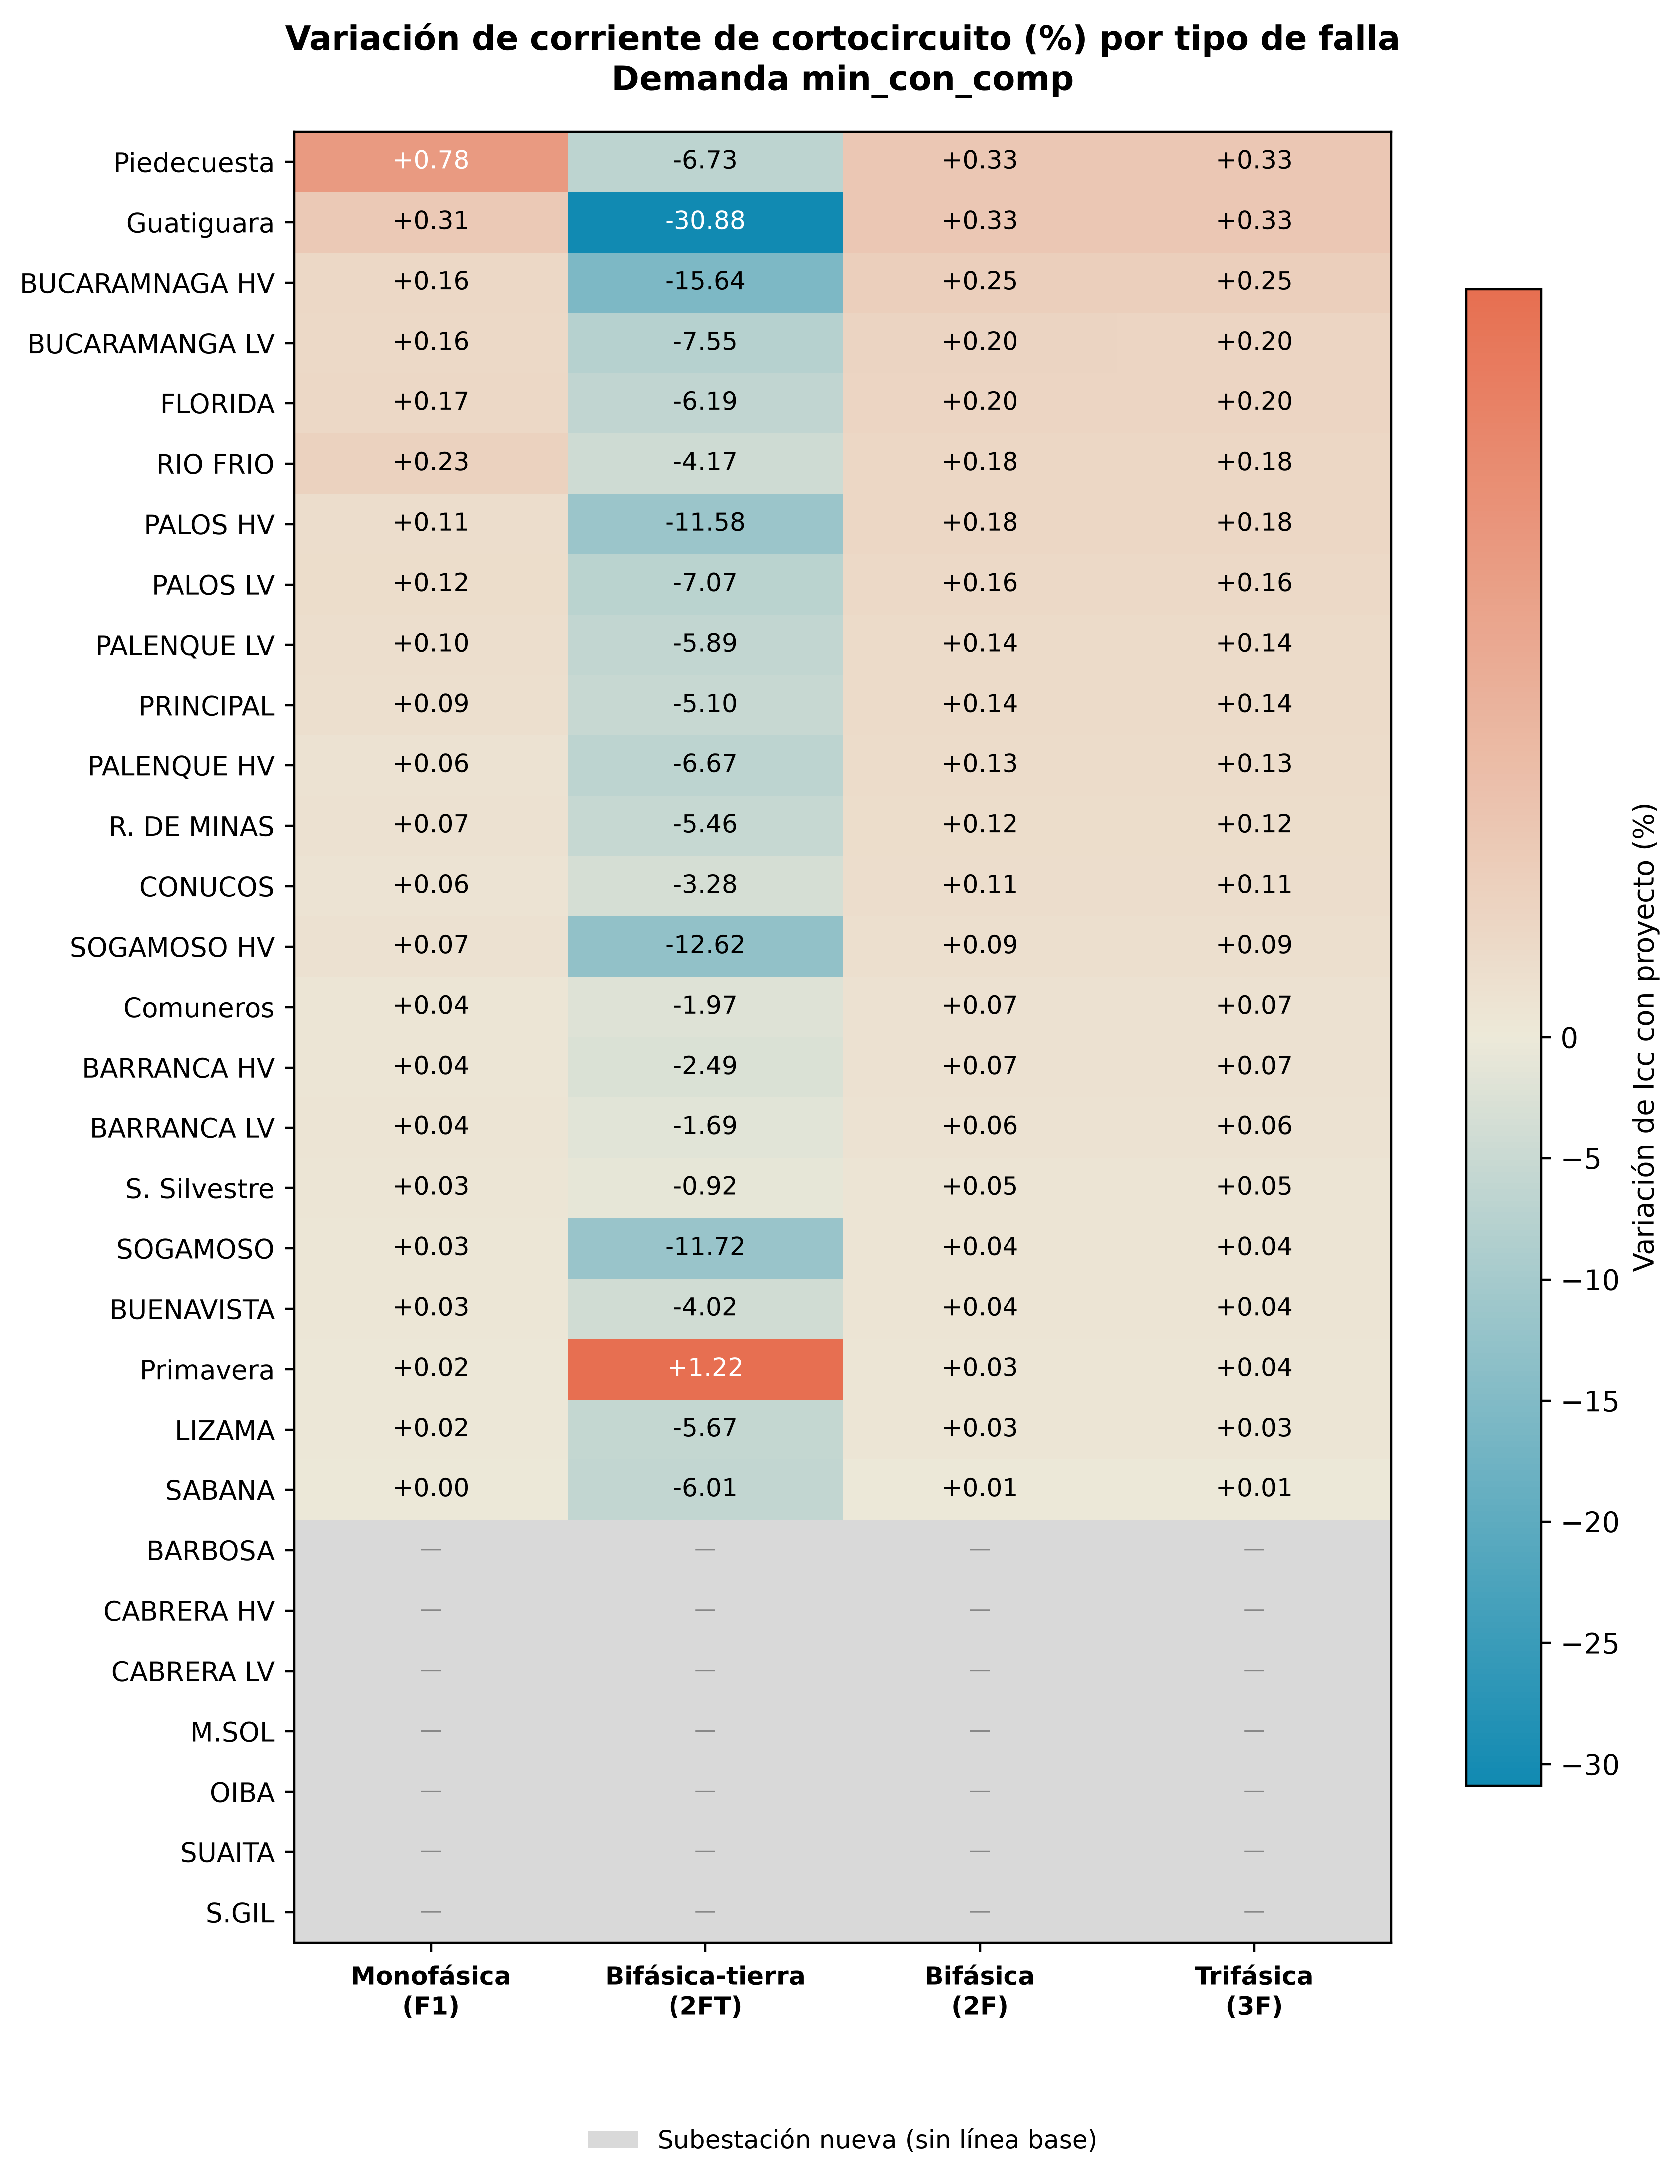
\includegraphics[width=0.75\linewidth]{variabminE1.png}
    \caption{Variación de corriente de cortocircuito Demanda mínima - E0 E1 compensado}
    \label{fig:var_Icc_demanda_min_E0_E1}
\end{figure}


\begin{figure}[H]
    \centering
    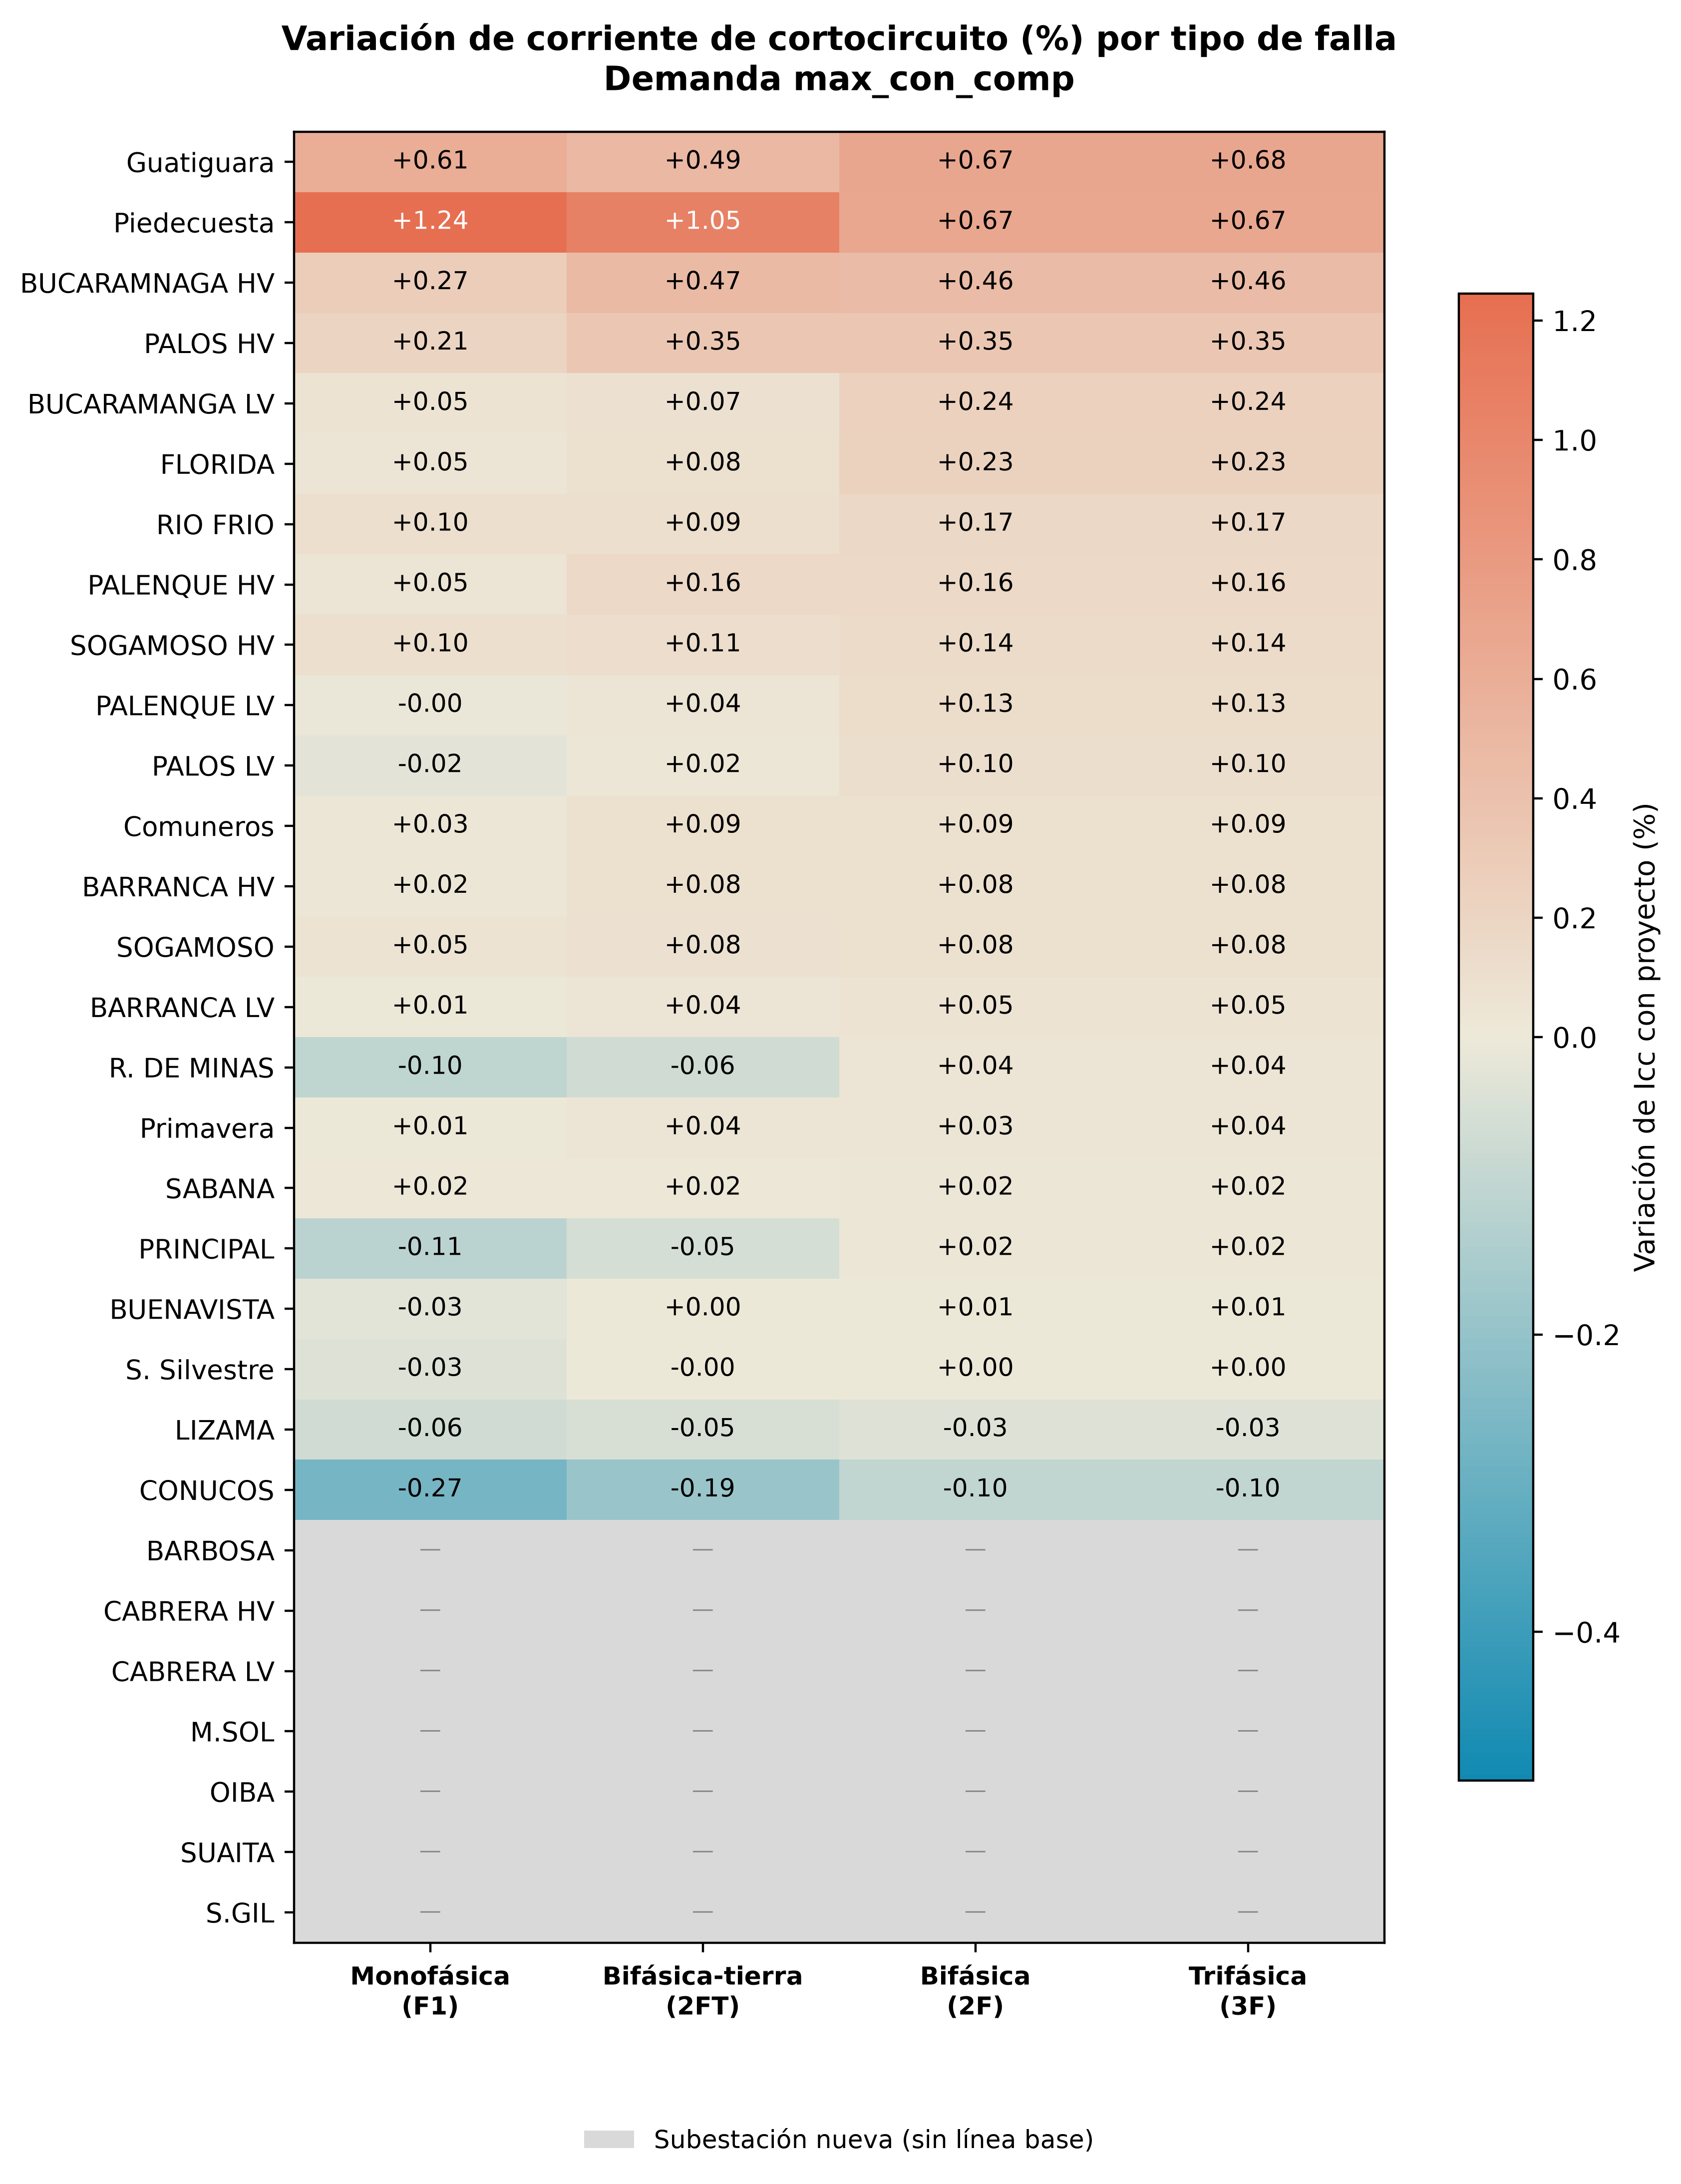
\includegraphics[width=0.75\linewidth]{variabmaxE1.png}
    \caption{Variación de corriente de cortocircuito Demanda máxima - E0 E1 compensado}
    \label{fig:var_Icc_demanda_max_E0_E1}
\end{figure}

\textbf{E0- E2}

\begin{figure}[H]
    \centering
    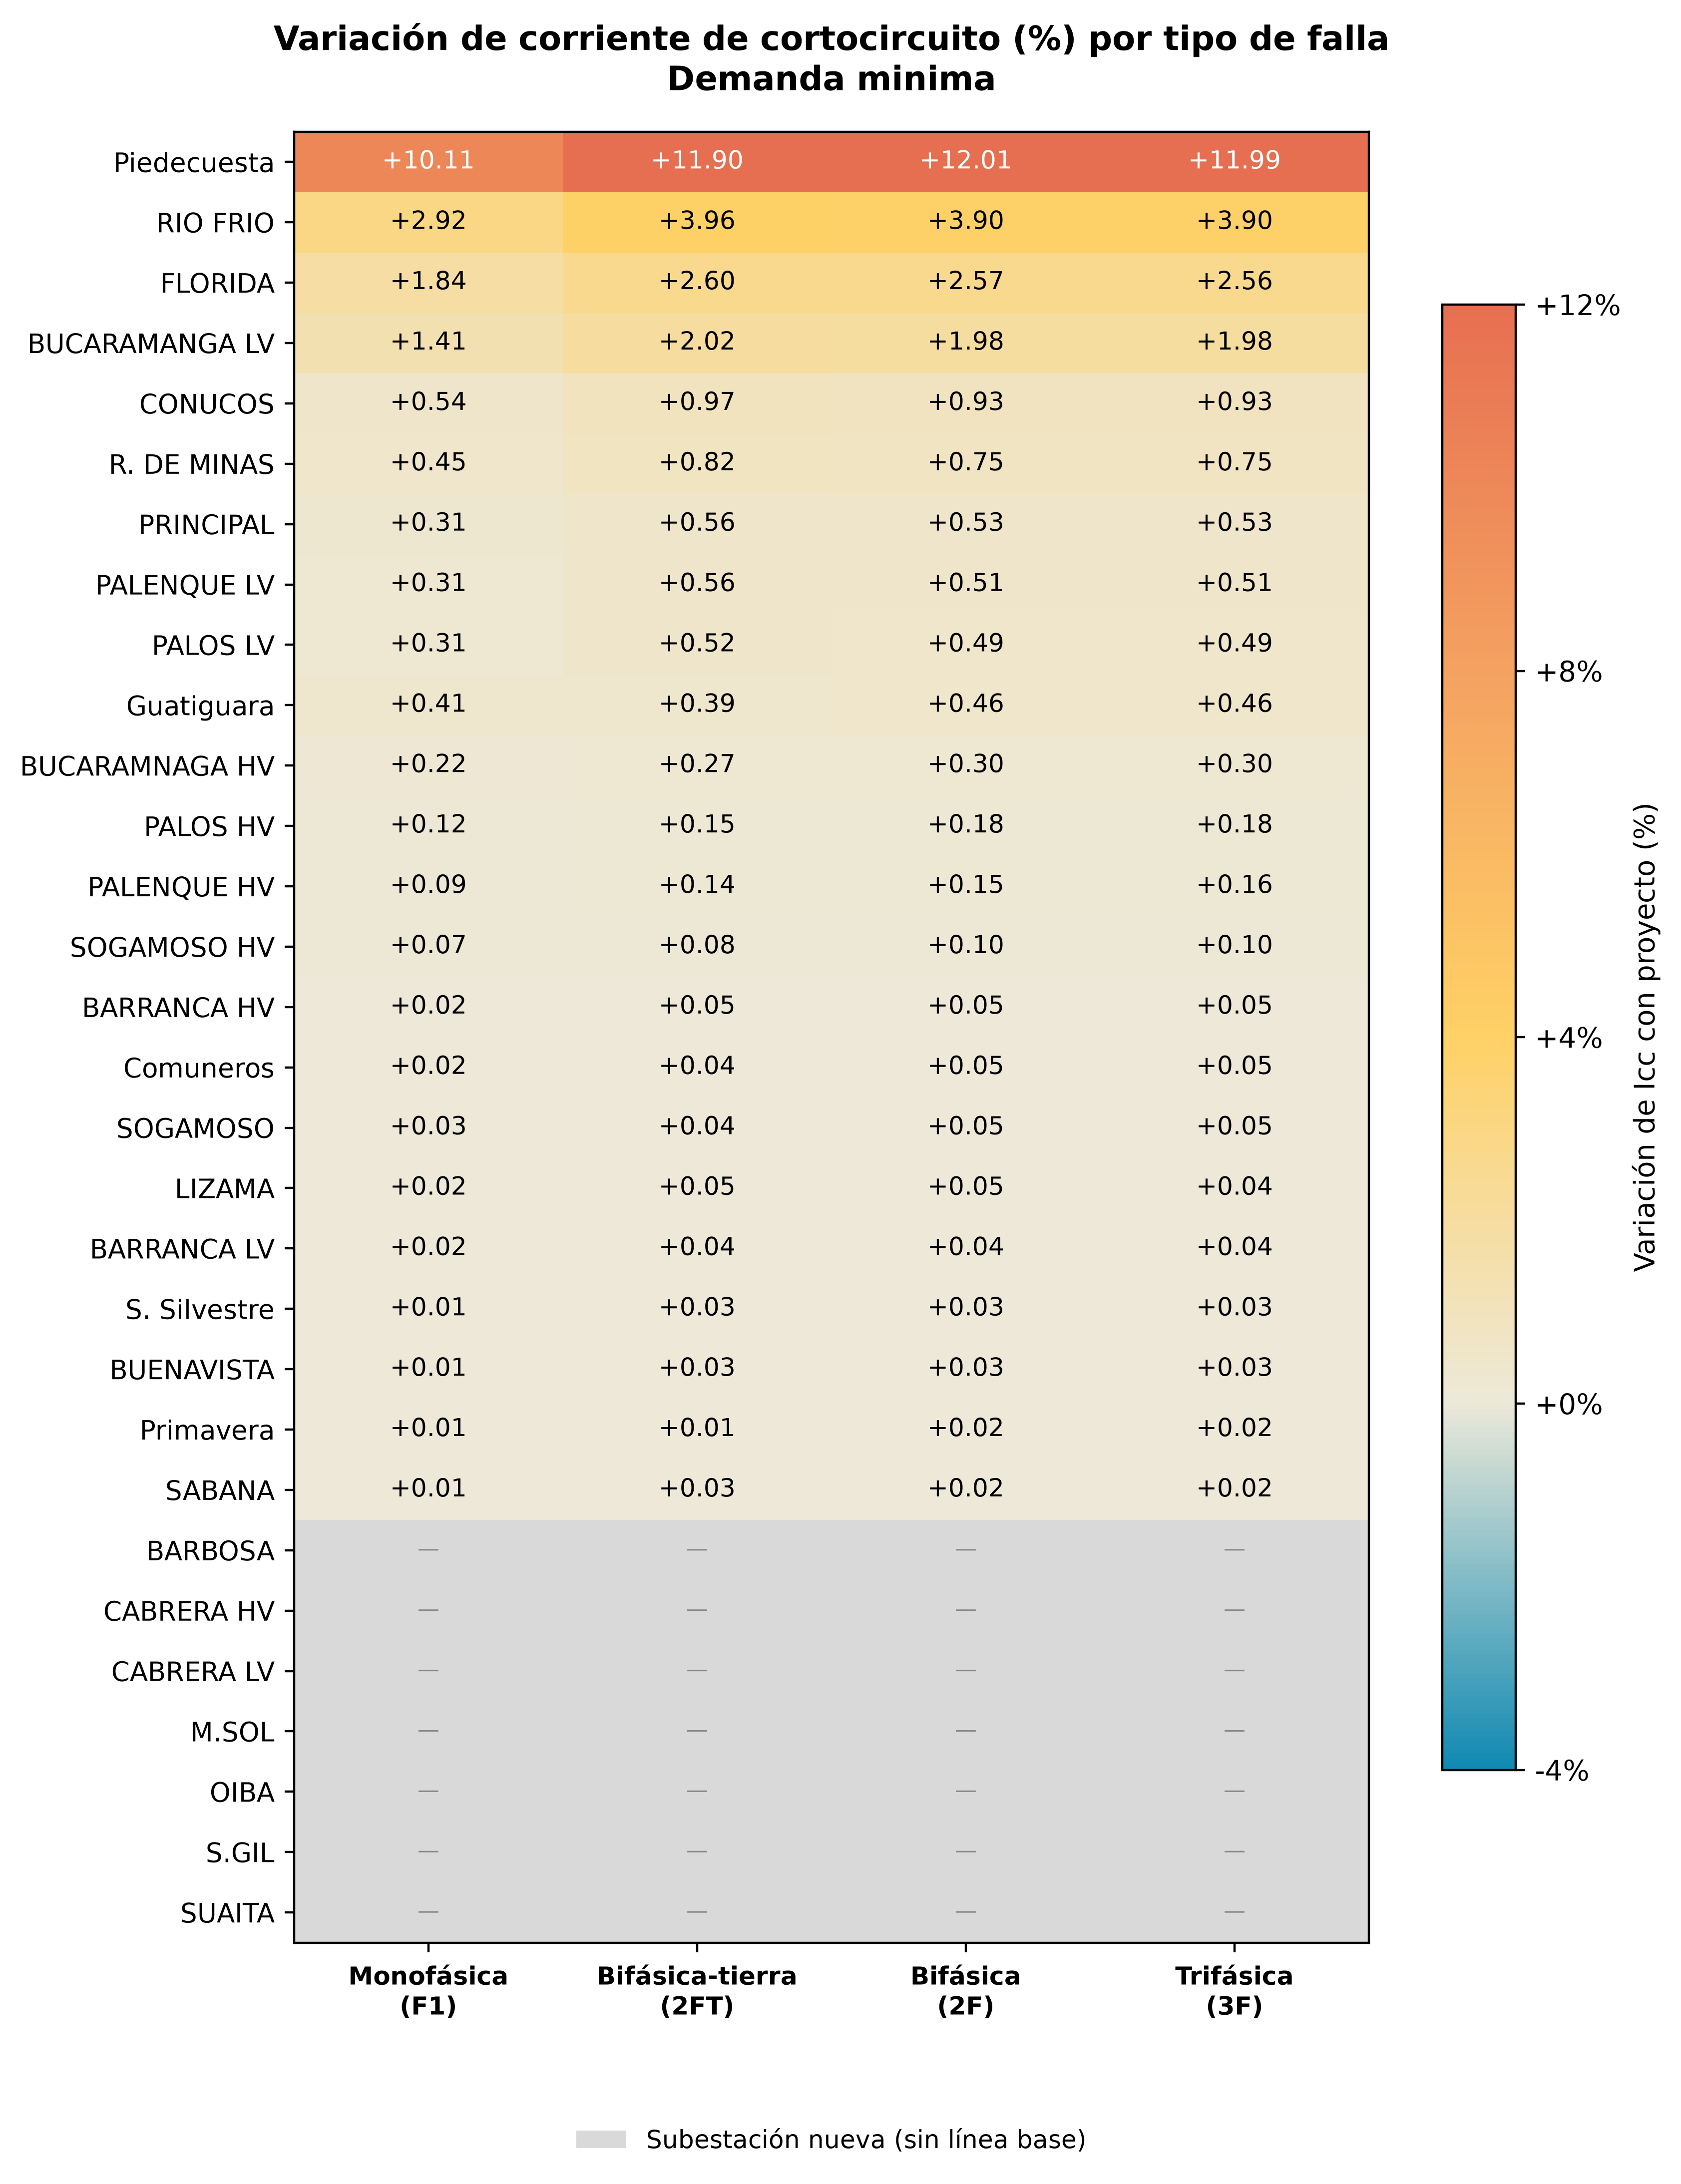
\includegraphics[width=0.75\linewidth]{variabmin.png}
    \caption{Variación de corriente de cortocircuito Demanda mínima - E0 E2}
    \label{fig:var_Icc_demanda_min_E0_E2}
\end{figure}


\begin{figure}[H]
    \centering
    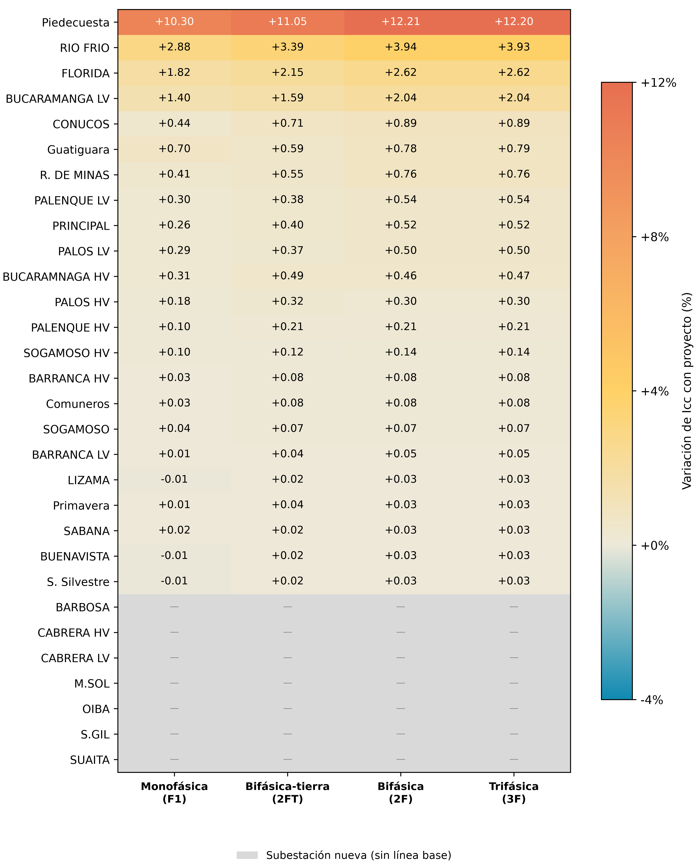
\includegraphics[width=0.75\linewidth]{variabilidad.png}
    \caption{Variación de corriente de cortocircuito Demanda máxima - E0 E2}
    \label{fig:placeholder}
\end{figure}

Al analizar los resultados de la variación porcentual de la corriente de cortocircuito tras la incorporación del proyecto, se observa que en términos generales los niveles de falla del sistema se mantienen estables y con variaciones muy bajas en la gran mayoría de subestaciones[3]. La única zona donde se presenta un impacto considerable es en la subestación Piedecuesta (115 kV y 220 kV), la cual registra los mayores incrementos de cortocircuito (entre +10.1\% y +12.2\%) debido a que constituye el punto directo de acople e interconexión de la nueva red[3]. En las subestaciones cercanas el incremento es leve y se reduce gradualmente a valores inferiores al +4\%, mientras que en los nodos más lejanos del proyecto la variabilidad es prácticamente nula o inferior al 0.03\%, confirmando que la entrada del proyecto no altera significativamente las condiciones de cortocircuito en el resto del sistema.

\subsection{Conclusiones y recomendaciones}
\begin{itemize}
    \item De acuerdo con los resultados obtenidos mediante el Método Completo de simulación, el tipo de falla que origina la mayor magnitud de corriente de cortocircuito inicial ($I_k''$) en la red es la \textbf{falla trifásica (3F)}, debido a que presenta la menor impedancia equivalente Thévenin del sistema. Respecto a las barras más críticas, la corriente de falla máxima de todo el modelo se concentra en los \textbf{bornes de generación de la Central Sogamoso (16.5 kV)} (superando los \textbf{240 kA}) por el aporte directo de sus tres unidades síncronas; mientras que, en el Sistema de Transmisión Nacional (220 kV), el nivel más elevado se registra en la barra de \textbf{Guatiguará 220 kV} (alcanzando hasta \textbf{58.6 kA}), y en el nivel de subtransmisión (115 kV) las mayores magnitudes se presentan en \textbf{Bucaramanga 115 kV} y \textbf{Piedecuesta 115 kV}, debido a la rigidez eléctrica que les otorgan las fuentes equivalentes de red  y los grandes bancos de transformación del área.

    \item Se comprobó que la incorporación de la Etapa 1 genera problemas de regulación de tensión en el sistema, presentándose niveles inferiores a 0,90 pu en las subestaciones Barbosa, Suaita, Oiba, Cabrera y San GiL, en donde la condición más desfavorable se presentó en la barra Barbosa 115 kV, con una tensión de 0,849 pu. Como medida correctiva, se determinó mediante simulaciones en DIgSILENT PowerFactory que una compensación reactiva mínima de 17 MVAr permite restablecer los niveles de tensión dentro de los límites establecidos y para su implementación se seleccionó un banco de capacitores comercial de 22,5 MVAr a 115 kV, verificándose su efectividad para corregir las condiciones de subtensión identificadas.
    \item La cargabilidad no es un problema generalizado, pero hay un elemento que merece atención aparte del proyecto. En las Figuras~\ref{fig:cargE0} y~\ref{fig:cargE1_sin_comp}, casi todas las líneas y transformadores se mantienen cómodamente bajo 70\%. La excepción es GUATIGUARA/BUCARAMANGA, que se mantiene entre 90--95\% en las tres etapas, independientemente del proyecto de protecciones; es decir, este representa un cuello de botella estructural preexistente que probablemente necesite su propio estudio de refuerzo o repotenciación, y no corresponde a una condición que el proyecto actual resuelva o empeore.
    \item El matiz del cortocircuito: sin compensación reactiva, el proyecto incrementa los niveles de falla modestamente en casi todo el sistema (0--3\%), con Piedecuesta destacándose con incrementos de +10--12\%. Por lo tanto, vale la pena verificar que los interruptores existentes en esta subestación continúen teniendo un margen de capacidad interruptiva suficiente. Con compensación (COMP), este aumento se reduce a valores cercanos a cero en demanda máxima ($\sim \pm 1\%$), lo cual indica que la compensación está cumpliendo su función de amortiguar el impacto del refuerzo sobre los niveles de cortocircuito. Sin embargo, en demanda mínima con compensación aparece un comportamiento diferente: la falla bifásica a tierra (2FT) disminuye hasta un 30\% en Guatiguará y de forma notable en varias otras barras, mientras que las demás fallas presentan variaciones reducidas. Una disminución de esta magnitud en un tipo de falla específico es tan relevante como un aumento, ya que, si algún relé de tierra fue calibrado considerando corrientes más altas, podría dejar de detectar fallas bajo esta condición, generando un posible problema de alcance insuficiente (\textit{under-reach}). Por esta razón, se recomienda revisar específicamente la coordinación de las protecciones de tierra para esta condición antes de dar por finalizado el estudio.

\end{itemize}





\newpage
\vspace*{0.1cm}

\begin{thebibliography}{1}


\bibliographystyle{IEEEtran}



\bibitem{ref1}
Consejo Nacional de Operación (CNO), ``Lineamientos para la elaboración y presentación de EACP del SIN colombiano,'' Subcomité de Protecciones, 2024. [En línea]. Disponible en: \url{http://35.193.94.55/solicitante/images/CNO\%201612\%20Lineamientos\%20para\%20la\%20elaboraci\%C3\%B3n\%20y\%20presentaci\%C3\%B3n\%20de\%20EACP\%20en\%20el\%20SIN.pdf}

\bibitem{ref2}
XM S.A. E.S.P., ``Demanda real por departamento,'' [En línea]. Disponible en: \url{https://sinergox.xm.com.co/dmnd/Paginas/Informes/DemandaRealDptoUNR.aspx}

\bibitem{ref3}
Comisión de Regulación de Energía y Gas (CREG), ``Concepto CREG 0000246 de 2024,'' 2024. [En línea]. Disponible en: \url{https://gestornormativo.creg.gov.co/gestor/entorno/docs/concepto_creg_0000246_2024.htm}

\bibitem{ref1}
Consejo Nacional de Operación (CNO), ``Lineamientos para la elaboración y presentación de EACP del SIN colombiano,'' Subcomité de Protecciones, 2024. [En línea]. Disponible en: \url{http://35.193.94.55/solicitante/images/CNO\%201612\%20Lineamientos\%20para\%20la\%20elaboraci\%C3\%B3n\%20y\%20presentaci\%C3\%B3n\%20de\%20EACP\%20en\%20el\%20SIN.pdf}

\bibitem{ref2}
EPRECSA, ``Bancos de capacitores para subestaciones de transmisión.'' [En línea]. Disponible en: \url{https://www.eprecsa.mx/bancos-de-capacitores-para-subestaciones-de-transmision/}
\end{thebibliography}

\newpage
\vspace*{0.1cm}

\section*{Anexo A}
\begin{figure}[H]
    \centering
    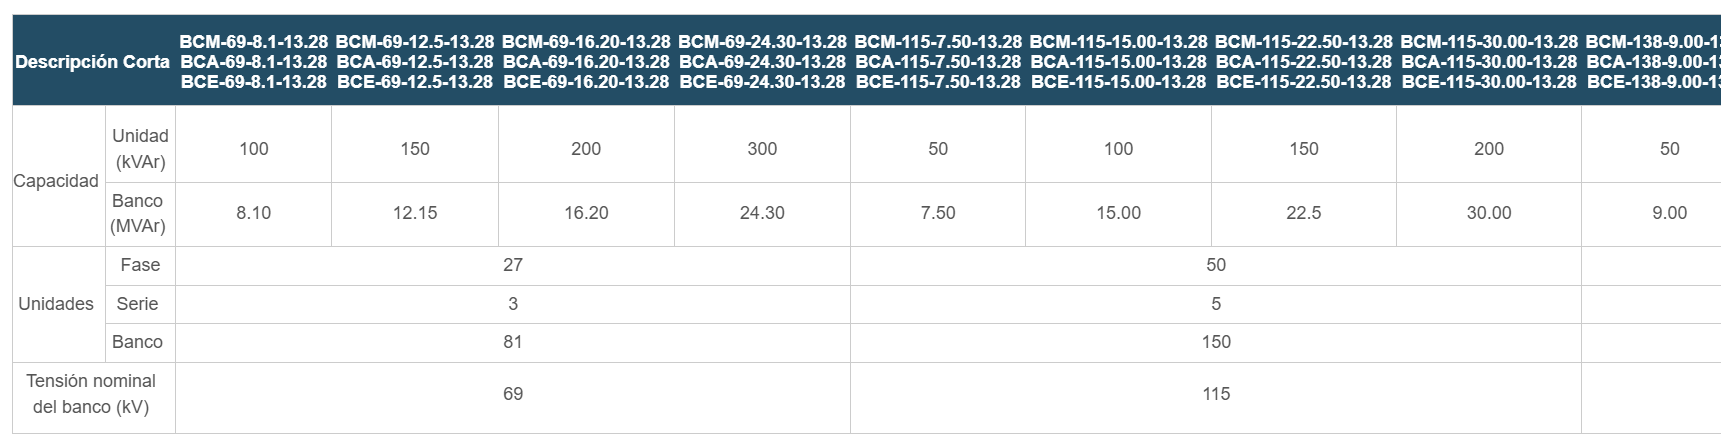
\includegraphics[width=\textwidth]{compensacion.png}
    \caption{Información comercial del banco de capacitores seleccionado}
    \label{fig:anexo_banco_capacitores}
\end{figure}

\end{document}
